\documentclass[11pt]{article}\usepackage[]{graphicx}\usepackage[]{xcolor}
% maxwidth is the original width if it is less than linewidth
% otherwise use linewidth (to make sure the graphics do not exceed the margin)
\makeatletter
\def\maxwidth{ %
  \ifdim\Gin@nat@width>\linewidth
    \linewidth
  \else
    \Gin@nat@width
  \fi
}
\makeatother

\definecolor{fgcolor}{rgb}{0.345, 0.345, 0.345}
\newcommand{\hlnum}[1]{\textcolor[rgb]{0.686,0.059,0.569}{#1}}%
\newcommand{\hlsng}[1]{\textcolor[rgb]{0.192,0.494,0.8}{#1}}%
\newcommand{\hlcom}[1]{\textcolor[rgb]{0.678,0.584,0.686}{\textit{#1}}}%
\newcommand{\hlopt}[1]{\textcolor[rgb]{0,0,0}{#1}}%
\newcommand{\hldef}[1]{\textcolor[rgb]{0.345,0.345,0.345}{#1}}%
\newcommand{\hlkwa}[1]{\textcolor[rgb]{0.161,0.373,0.58}{\textbf{#1}}}%
\newcommand{\hlkwb}[1]{\textcolor[rgb]{0.69,0.353,0.396}{#1}}%
\newcommand{\hlkwc}[1]{\textcolor[rgb]{0.333,0.667,0.333}{#1}}%
\newcommand{\hlkwd}[1]{\textcolor[rgb]{0.737,0.353,0.396}{\textbf{#1}}}%
\let\hlipl\hlkwb

\usepackage{framed}
\makeatletter
\newenvironment{kframe}{%
 \def\at@end@of@kframe{}%
 \ifinner\ifhmode%
  \def\at@end@of@kframe{\end{minipage}}%
  \begin{minipage}{\columnwidth}%
 \fi\fi%
 \def\FrameCommand##1{\hskip\@totalleftmargin \hskip-\fboxsep
 \colorbox{shadecolor}{##1}\hskip-\fboxsep
     % There is no \\@totalrightmargin, so:
     \hskip-\linewidth \hskip-\@totalleftmargin \hskip\columnwidth}%
 \MakeFramed {\advance\hsize-\width
   \@totalleftmargin\z@ \linewidth\hsize
   \@setminipage}}%
 {\par\unskip\endMakeFramed%
 \at@end@of@kframe}
\makeatother

\definecolor{shadecolor}{rgb}{.97, .97, .97}
\definecolor{messagecolor}{rgb}{0, 0, 0}
\definecolor{warningcolor}{rgb}{1, 0, 1}
\definecolor{errorcolor}{rgb}{1, 0, 0}
\newenvironment{knitrout}{}{} % an empty environment to be redefined in TeX

\usepackage{alltt}

% --- Packages for math & formatting ---
\usepackage{amsmath, amssymb, amsthm} % advanced math
\usepackage{listings}                  % code formatting
\usepackage{xcolor}                     % color for code
\usepackage{graphicx}                   % include figures
\usepackage{hyperref}                   % clickable links
\usepackage{authblk}                    % author affiliations
\usepackage[margin=1in]{geometry}
\usepackage{fvextra} % better verbatim with line wrapping
\usepackage{float}

% --- Configure code display ---
\lstset{
  language=R,
  basicstyle=\ttfamily\small,
  numbers=left,
  stepnumber=1,
  numbersep=5pt,
  frame=single,
  backgroundcolor=\color{gray!10},
  breaklines=true,
  captionpos=b
}

% --- Theorem environment ---
\newtheorem{theorem}{Theorem}
\newtheorem{lemma}{Lemma}

% --- New commands ---
\newcommand*\mean[1]{\overline{#1}}
\newcommand{\var}{\text{var}}
\newcommand{\cov}{\text{cov}}
\newcommand{\cor}{\text{cor}}
\newcommand{\Rp}{\text{Re}}
\newcommand{\E}{\text{E}}
\newcommand{\ltsgr}{\text{ltsgr}}
\newcommand{\expit}{\text{expit}}
\newcommand{\logit}{\text{logit}}

% --- Header material ---
\title{How to fit models with species occurrence data using \texttt{xsdm}}
\author[1]{Daniel C. Reuman}
\author[1]{Angel Lu\'{i}s Robles Fern\'{a}ndez}
\affil[1]{Department of Ecology and Evolutionary Biology and Center for Ecological Research,
University of Kansas}
\date{}

% --- Make Sweave code/output blocks obey text margins and wrap nicely ---
\DefineVerbatimEnvironment{Sinput}{Verbatim}{
  fontsize=\small,
  xleftmargin=0pt,
  xrightmargin=0pt,
  breaklines=true,
  breakanywhere=true,
  commandchars=\\\{\}
}

\DefineVerbatimEnvironment{Soutput}{Verbatim}{
  fontsize=\small,
  xleftmargin=0pt,
  xrightmargin=0pt,
  breaklines=true,
  breakanywhere=true,
  commandchars=\\\{\}
}

% Optional: if you have Scode blocks too
\DefineVerbatimEnvironment{Scode}{Verbatim}{
  fontsize=\small,
  xleftmargin=0pt,
  xrightmargin=0pt,
  breaklines=true,
  breakanywhere=true,
  commandchars=\\\{\}
}

% --- start the doc ---
\IfFileExists{upquote.sty}{\usepackage{upquote}}{}
\begin{document}






\maketitle

\begin{abstract}
\noindent After reading the document entitled "The xsdm model", this document
introduces the statistically and computationally sophisticated user to the 
main functions of the \texttt{xsdm} package. The package implements a frequentist 
analysis of the xsdm model. This document should get the user to the point
of maximizing the likelihood of the model and profiling in ``easy'' cases, 
with callouts to
several troubleshooting documents about what to do when the process does
not go smoothly. Alternative fitted models can also be compared by AIC or another
criterion. The example worked out here is for a virtual species (i.e., generated 
data), so we also demonstrate that fitting an xsdm model can recover the true
parameters if model mis-specification is not an issue.
\end{abstract}

\section{Introduction to the running example used throughout this document}

This manual uses a small built-in example included with the \texttt{xsdm} R 
package to illustrate a baseline workflow. The example contains (i) an
occurrence table for a virtual species, and (ii) two environmental
\texttt{terra} raster time series representing CHELSA-derived 
bioclimatic variables for a region of interest over 39 years.

Load the data and get oriented to the first bioclimatic variable, which is mean annual temperature
in units of $100 \times ^\circ$C for 39 years for a particular region of interest. 
And make it units of $^\circ$C: 
\begin{knitrout}
\definecolor{shadecolor}{rgb}{0.969, 0.969, 0.969}\color{fgcolor}\begin{kframe}
\begin{alltt}
\hlkwd{library}\hldef{(xsdm)}
\hlkwd{library}\hldef{(terra)}
\hlcom{#This is for better display}
\hlkwd{options}\hldef{(}\hlkwc{digits} \hldef{=} \hlnum{3}\hldef{)}
\hlkwd{data}\hldef{(}\hlsng{"example_1"}\hldef{)}
\hldef{bio_1} \hlkwb{<-} \hldef{terra}\hlopt{::}\hlkwd{unwrap}\hldef{(example_1}\hlopt{$}\hldef{bio01)}
\hlkwd{class}\hldef{(bio_1)}
\end{alltt}
\begin{verbatim}
## [1] "SpatRaster"
## attr(,"package")
## [1] "terra"
\end{verbatim}
\begin{alltt}
\hlkwd{dim}\hldef{(bio_1)}
\end{alltt}
\begin{verbatim}
## [1] 128 123  39
\end{verbatim}
\begin{alltt}
\hldef{mm} \hlkwb{<-} \hldef{terra}\hlopt{::}\hlkwd{global}\hldef{(bio_1,}\hlkwc{fun}\hldef{=}\hlkwd{c}\hldef{(}\hlsng{"min"}\hldef{,}\hlsng{"max"}\hldef{))}
\hlkwd{min}\hldef{(mm}\hlopt{$}\hldef{min)} \hlcom{#global min over all years and all locations}
\end{alltt}
\begin{verbatim}
## [1] -154
\end{verbatim}
\begin{alltt}
\hlkwd{max}\hldef{(mm}\hlopt{$}\hldef{max)} \hlcom{#global max}
\end{alltt}
\begin{verbatim}
## [1] 2061
\end{verbatim}
\begin{alltt}
\hldef{bio_1} \hlkwb{<-} \hldef{bio_1}\hlopt{/}\hlnum{100} \hlcom{#Make it degrees C}
\end{alltt}
\end{kframe}
\end{knitrout}

Now load the second environmental variable, which is annual total precipitation, in units of kg/m$^2$, for
the same 39 years and the same region of interest:
\begin{knitrout}
\definecolor{shadecolor}{rgb}{0.969, 0.969, 0.969}\color{fgcolor}\begin{kframe}
\begin{alltt}
\hldef{bio_12} \hlkwb{<-} \hldef{terra}\hlopt{::}\hlkwd{unwrap}\hldef{(example_1}\hlopt{$}\hldef{bio12)}
\hlkwd{class}\hldef{(bio_12)}
\end{alltt}
\begin{verbatim}
## [1] "SpatRaster"
## attr(,"package")
## [1] "terra"
\end{verbatim}
\begin{alltt}
\hlkwd{dim}\hldef{(bio_12)}
\end{alltt}
\begin{verbatim}
## [1] 128 123  39
\end{verbatim}
\begin{alltt}
\hldef{mm} \hlkwb{<-}  \hldef{terra}\hlopt{::}\hlkwd{global}\hldef{(bio_12,}\hlkwc{fun}\hldef{=}\hlkwd{c}\hldef{(}\hlsng{"min"}\hldef{,}\hlsng{"max"}\hldef{))}
\hlkwd{min}\hldef{(mm}\hlopt{$}\hldef{min)} \hlcom{#again the global min, all years and locations}
\end{alltt}
\begin{verbatim}
## [1] 45
\end{verbatim}
\begin{alltt}
\hlkwd{max}\hldef{(mm}\hlopt{$}\hldef{max)} \hlcom{#global max}
\end{alltt}
\begin{verbatim}
## [1] 1761
\end{verbatim}
\end{kframe}
\end{knitrout}

If the scales of your environmental variables are vastly different, it can cause problems
with optimization (see the document ``Troubleshooting: Optimization problems related to scaling").
So we change the units for precipitation to make the range of values similar to those for temperature.
Now the units are going to be dg/m$^2$:
\begin{knitrout}
\definecolor{shadecolor}{rgb}{0.969, 0.969, 0.969}\color{fgcolor}\begin{kframe}
\begin{alltt}
\hldef{bio_12} \hlkwb{=} \hldef{bio_12}\hlopt{/}\hlnum{100}
\hldef{mm} \hlkwb{<-} \hldef{terra}\hlopt{::}\hlkwd{global}\hldef{(bio_1,}\hlkwc{fun}\hldef{=}\hlkwd{c}\hldef{(}\hlsng{"min"}\hldef{,}\hlsng{"max"}\hldef{))}
\hlkwd{min}\hldef{(mm}\hlopt{$}\hldef{min)}
\end{alltt}
\begin{verbatim}
## [1] -1.54
\end{verbatim}
\begin{alltt}
\hlkwd{max}\hldef{(mm}\hlopt{$}\hldef{max)}
\end{alltt}
\begin{verbatim}
## [1] 20.6
\end{verbatim}
\begin{alltt}
\hldef{mm} \hlkwb{<-} \hldef{terra}\hlopt{::}\hlkwd{global}\hldef{(bio_12,}\hlkwc{fun}\hldef{=}\hlkwd{c}\hldef{(}\hlsng{"min"}\hldef{,}\hlsng{"max"}\hldef{))}
\hlkwd{min}\hldef{(mm}\hlopt{$}\hldef{min)}
\end{alltt}
\begin{verbatim}
## [1] 0.45
\end{verbatim}
\begin{alltt}
\hlkwd{max}\hldef{(mm}\hlopt{$}\hldef{max)}
\end{alltt}
\begin{verbatim}
## [1] 17.6
\end{verbatim}
\end{kframe}
\end{knitrout}

Next load data on detections and non-detections/pseudo-absences for a species:
\begin{knitrout}
\definecolor{shadecolor}{rgb}{0.969, 0.969, 0.969}\color{fgcolor}\begin{kframe}
\begin{alltt}
\hldef{d} \hlkwb{<-} \hldef{example_1}\hlopt{$}\hldef{occ_df}
\hlkwd{class}\hldef{(d)}
\end{alltt}
\begin{verbatim}
## [1] "tbl_df"     "tbl"        "data.frame"
\end{verbatim}
\begin{alltt}
\hlkwd{dim}\hldef{(d)}
\end{alltt}
\begin{verbatim}
## [1] 4000    4
\end{verbatim}
\begin{alltt}
\hlkwd{head}\hldef{(d)}
\end{alltt}
\begin{verbatim}
## # A tibble: 6 x 4
##   name                   lon      lat presence
##   <chr>                <dbl>    <dbl>    <int>
## 1 Species virtualis -1108723 1402222.        1
## 2 Species virtualis  -883723 1402222.        0
## 3 Species virtualis  -808723 1422222.        1
## 4 Species virtualis -1168723 1552222.        0
## 5 Species virtualis -1028723 1437222.        0
## 6 Species virtualis  -948723 1452222.        1
\end{verbatim}
\begin{alltt}
\hlkwd{sum}\hldef{(d}\hlopt{$}\hldef{presence} \hlopt{==} \hlnum{1}\hldef{)}
\end{alltt}
\begin{verbatim}
## [1] 1609
\end{verbatim}
\end{kframe}
\end{knitrout}
%DAN: Note, this chunk will change when the data for the species become wrapped in the package 

Now take a basic look at the environmental variables and the species data, just to see what we
have. Start
by getting the means through time of the environmental time series and plotting:
\begin{knitrout}
\definecolor{shadecolor}{rgb}{0.969, 0.969, 0.969}\color{fgcolor}\begin{kframe}
\begin{alltt}
\hldef{m_bio_1} \hlkwb{=} \hldef{terra}\hlopt{::}\hlkwd{app}\hldef{(bio_1,mean)}
\hldef{m_bio_12} \hlkwb{=} \hldef{terra}\hlopt{::}\hlkwd{app}\hldef{(bio_12,mean)}
\hlkwd{par}\hldef{(}\hlkwc{mfrow}\hldef{=}\hlkwd{c}\hldef{(}\hlnum{1}\hldef{,}\hlnum{2}\hldef{))}
\hldef{terra}\hlopt{::}\hlkwd{plot}\hldef{(m_bio_1,}\hlkwc{axes}\hldef{=}\hlnum{TRUE}\hldef{,}\hlkwc{main}\hldef{=}\hlsng{"Mean, bio1"}\hldef{,}\hlkwc{xlab}\hldef{=}\hlsng{"x"}\hldef{,}\hlkwc{ylab}\hldef{=}\hlsng{"y"}\hldef{,}\hlkwc{legend}\hldef{=}\hlnum{TRUE}\hldef{)}
\hldef{terra}\hlopt{::}\hlkwd{plot}\hldef{(m_bio_12,}\hlkwc{axes}\hldef{=}\hlnum{TRUE}\hldef{,}\hlkwc{main}\hldef{=}\hlsng{"Mean, bio12"}\hldef{,}\hlkwc{xlab}\hldef{=}\hlsng{"x"}\hldef{,}\hlkwc{ylab}\hldef{=}\hlsng{"y"}\hldef{,}\hlkwc{legend}\hldef{=}\hlnum{TRUE}\hldef{)}
\end{alltt}
\end{kframe}
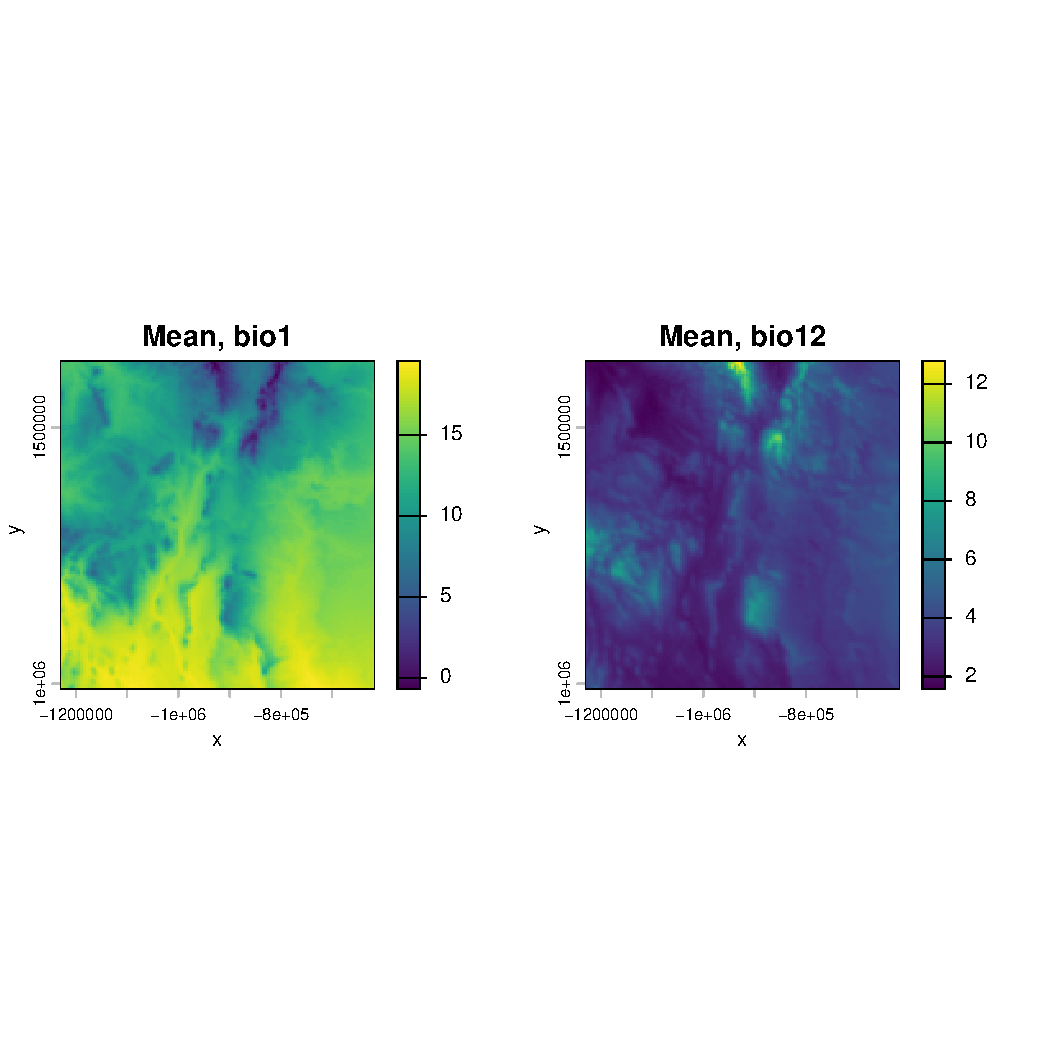
\includegraphics[width=\maxwidth]{figure/look_at_data_01-1} 
\end{knitrout}
%DAN: The spacing here is bad (way too much whitespace), and the sizing of the figures is sub-optimal
%They should be bigger. Not sure how to fix.

\noindent Now do the same for standard deviations:
\begin{knitrout}
\definecolor{shadecolor}{rgb}{0.969, 0.969, 0.969}\color{fgcolor}\begin{kframe}
\begin{alltt}
\hldef{sd_bio_1} \hlkwb{=} \hldef{terra}\hlopt{::}\hlkwd{app}\hldef{(bio_1,sd)}
\hldef{sd_bio_12} \hlkwb{=} \hldef{terra}\hlopt{::}\hlkwd{app}\hldef{(bio_12,sd)}
\hlkwd{par}\hldef{(}\hlkwc{mfrow}\hldef{=}\hlkwd{c}\hldef{(}\hlnum{1}\hldef{,}\hlnum{2}\hldef{))}
\hldef{terra}\hlopt{::}\hlkwd{plot}\hldef{(sd_bio_1,}\hlkwc{axes}\hldef{=}\hlnum{TRUE}\hldef{,}\hlkwc{main}\hldef{=}\hlsng{"SD, bio1"}\hldef{,}\hlkwc{xlab}\hldef{=}\hlsng{"x"}\hldef{,}\hlkwc{ylab}\hldef{=}\hlsng{"y"}\hldef{,}\hlkwc{legend}\hldef{=}\hlnum{TRUE}\hldef{)}
\hldef{terra}\hlopt{::}\hlkwd{plot}\hldef{(sd_bio_12,}\hlkwc{axes}\hldef{=}\hlnum{TRUE}\hldef{,}\hlkwc{main}\hldef{=}\hlsng{"SD, bio12"}\hldef{,}\hlkwc{xlab}\hldef{=}\hlsng{"x"}\hldef{,}\hlkwc{ylab}\hldef{=}\hlsng{"y"}\hldef{,}\hlkwc{legend}\hldef{=}\hlnum{TRUE}\hldef{)}
\end{alltt}
\end{kframe}
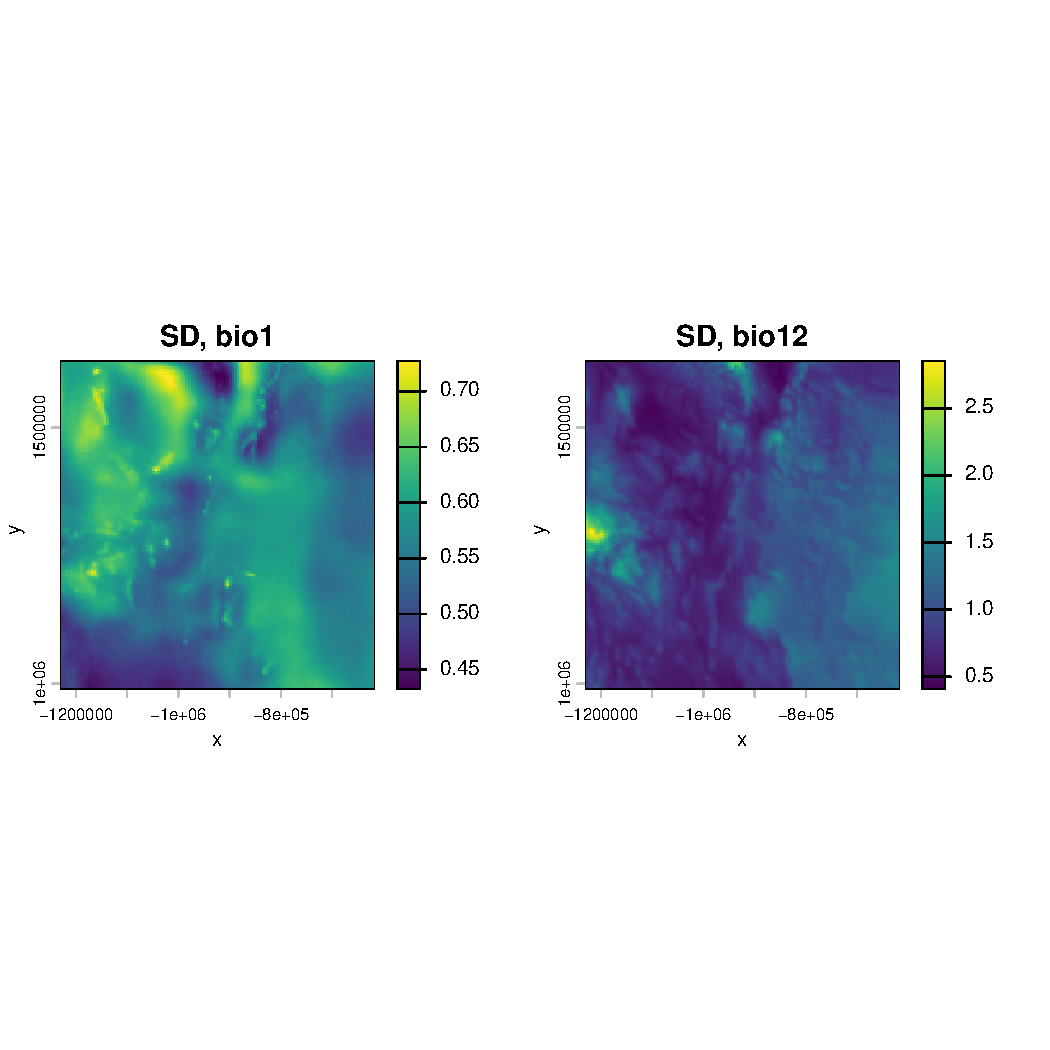
\includegraphics[width=\maxwidth]{figure/look_at_data_02-1} 
\end{knitrout}

\noindent Now plot the species detections and non-detections/pseudo-absences on a backdrop of the mean of bio 1:
\begin{knitrout}
\definecolor{shadecolor}{rgb}{0.969, 0.969, 0.969}\color{fgcolor}\begin{kframe}
\begin{alltt}
\hldef{d} \hlkwb{<-} \hlkwd{as.data.frame}\hldef{(d)}
\hldef{pts_0} \hlkwb{<-} \hldef{terra}\hlopt{::}\hlkwd{vect}\hldef{(d[d}\hlopt{$}\hldef{presence} \hlopt{==} \hlnum{0}\hldef{, ],}
                     \hlkwc{geom}\hldef{=}\hlkwd{c}\hldef{(}\hlsng{"lon"}\hldef{,}\hlsng{"lat"}\hldef{),}
                     \hlkwc{crs}\hldef{=terra}\hlopt{::}\hlkwd{crs}\hldef{(m_bio_1))}
\hldef{pts_1} \hlkwb{<-} \hldef{terra}\hlopt{::}\hlkwd{vect}\hldef{(d[d}\hlopt{$}\hldef{presence} \hlopt{==} \hlnum{1}\hldef{, ],}
                     \hlkwc{geom} \hldef{=} \hlkwd{c}\hldef{(}\hlsng{"lon"}\hldef{,}\hlsng{"lat"}\hldef{),}
                     \hlkwc{crs}\hldef{=terra}\hlopt{::}\hlkwd{crs}\hldef{(m_bio_1))}
\hlkwd{par}\hldef{(}\hlkwc{mfrow}\hldef{=}\hlkwd{c}\hldef{(}\hlnum{1}\hldef{,}\hlnum{2}\hldef{))}
\hldef{terra}\hlopt{::}\hlkwd{plot}\hldef{(m_bio_1,}
            \hlkwc{axes} \hldef{=} \hlnum{TRUE}\hldef{,}
            \hlkwc{main} \hldef{=} \hlsng{"Non-detections"}\hldef{,}
            \hlkwc{xlab}\hldef{=}\hlsng{"x"}\hldef{,}
            \hlkwc{ylab}\hldef{=}\hlsng{"y"}\hldef{,}
            \hlkwc{legend} \hldef{=} \hlnum{TRUE}\hldef{)}
\hldef{terra}\hlopt{::}\hlkwd{plot}\hldef{(pts_0,} \hlkwc{add}\hldef{=}\hlnum{TRUE}\hldef{,}\hlkwc{col}\hldef{=}\hlsng{"black"}\hldef{,}\hlkwc{pch}\hldef{=}\hlnum{20}\hldef{,}\hlkwc{cex}\hldef{=}\hlnum{.2}\hldef{)}
\hldef{terra}\hlopt{::}\hlkwd{plot}\hldef{(m_bio_1,}
            \hlkwc{axes} \hldef{=} \hlnum{TRUE}\hldef{,}
            \hlkwc{main} \hldef{=} \hlsng{"Detections"}\hldef{,}
            \hlkwc{xlab} \hldef{=} \hlsng{"x"}\hldef{,}
            \hlkwc{ylab} \hldef{=} \hlsng{"y"}\hldef{,}
            \hlkwc{legend} \hldef{=} \hlnum{TRUE}\hldef{)}
\hldef{terra}\hlopt{::}\hlkwd{plot}\hldef{(pts_1,} \hlkwc{add}\hldef{=}\hlnum{TRUE}\hldef{,}\hlkwc{col}\hldef{=}\hlsng{"black"}\hldef{,}\hlkwc{pch}\hldef{=}\hlnum{20}\hldef{,}\hlkwc{cex}\hldef{=}\hlnum{.2}\hldef{)}
\end{alltt}
\end{kframe}
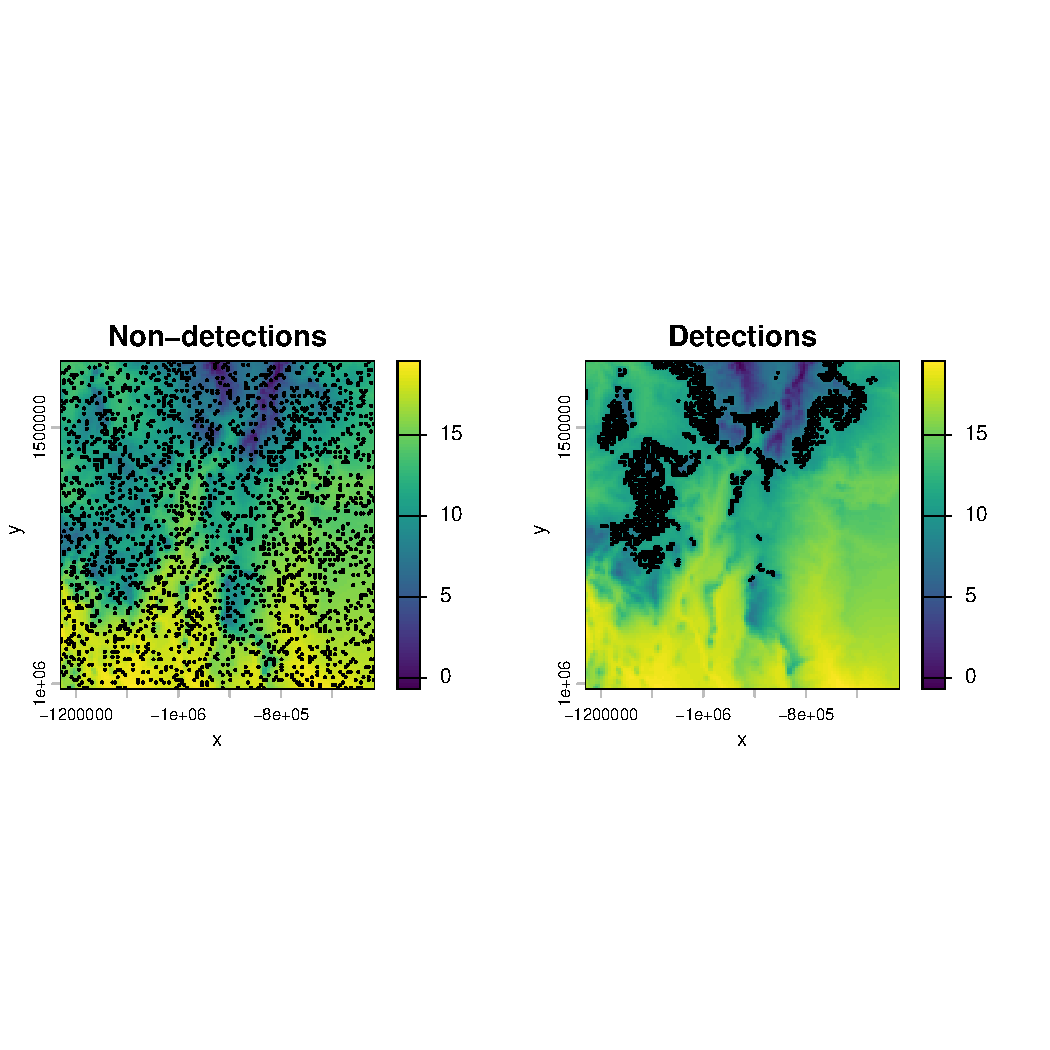
\includegraphics[width=\maxwidth]{figure/look_at_data_03-1} 
\end{knitrout}

The fitting tools offered by \texttt{xsdm} use a more succinct version of the data,
since only the environmental time series at the locations for which there is a 
detection or a non-detection/pseudo-absence matter; though we will return to using 
rasters after fitting and model selection. So, for now, we cut out only those
time series at the species locations and store them in an array using the convenience 
function \texttt{env\_data\_array}:

\begin{knitrout}
\definecolor{shadecolor}{rgb}{0.969, 0.969, 0.969}\color{fgcolor}\begin{kframe}
\begin{alltt}
\hldef{env_data} \hlkwb{<-} \hlkwd{list}\hldef{(}\hlkwc{bio_1} \hldef{= bio_1,} \hlkwc{bio_12} \hldef{= bio_12)}  \hlcom{# order defines variable 1 and 2}
\hldef{env_array} \hlkwb{<-} \hlkwd{env_data_array}\hldef{(env_data, d)}  \hlcom{# (n locations) x (time) x (p vars)}
\hlkwd{class}\hldef{(env_array)}
\end{alltt}
\begin{verbatim}
## [1] "array"
\end{verbatim}
\begin{alltt}
\hlkwd{dim}\hldef{(env_array)}
\end{alltt}
\begin{verbatim}
## [1] 4000   39    2
\end{verbatim}
\end{kframe}
\end{knitrout}

\noindent And we pull out the presences/pseudo-absences as a binary vector:
\begin{knitrout}
\definecolor{shadecolor}{rgb}{0.969, 0.969, 0.969}\color{fgcolor}\begin{kframe}
\begin{alltt}
\hldef{occ} \hlkwb{<-} \hldef{d}\hlopt{$}\hldef{presence}
\hlkwd{length}\hldef{(occ)}
\end{alltt}
\begin{verbatim}
## [1] 4000
\end{verbatim}
\end{kframe}
\end{knitrout}

\noindent Now we are ready to think about how the xsdm model applies to our data.

\section{Evaluating the likelihood}

The xsdm model's likelihood function is described in the document "The xsdm model",
where model parameter are also described in detail. Parameters are:
\begin{itemize}
\item $\vec{\mu}$, which encodes ideal values for population growth 
of the two environmental variables (a length-2 vector for the present 
scenario of two environmental variables, unconstrained values); 
\item $\tilde{\vec{\sigma}}_L$, which has to do with breadth of the growth-environment
function ``to the left'' with respect to two basis vectors (a length-2 vector for our case,
positive entries);
%Note, here I am NOT saying these can be Inf, will cover the boundary models in another doc
\item $\tilde{\vec{\sigma}}_R$, which is similar but ``to the right'' (a length-2 vector,
positive entries);
\item $\tilde{c}$ and $p_d$, which relate to species detection (scalars, $\tilde{c}$ is 
unconstrained and $0<p_d\leq 1$); and
\item $O$, which is an orthogonal matrix which 
describes the basis vectors mentioned above ($2 \times 2$ for the present example, must be
orthogonal, i.e., $OO^{\tau}=I$ for $\tau$ the transpose).
\end{itemize}
In code, the above parameters are denoted \texttt{mu}, \texttt{sigltil}, \texttt{sigrtil},
\texttt{ctil}, \texttt{pd}, and \texttt{o\_mat}.

The likelihood is coded as \texttt{loglik\_bio}, so as an introduction to the function 
let's evaluate it at a haphazardly chosen set of parameters:
\begin{knitrout}
\definecolor{shadecolor}{rgb}{0.969, 0.969, 0.969}\color{fgcolor}\begin{kframe}
\begin{alltt}
\hldef{mu} \hlkwb{<-} \hlkwd{c}\hldef{(}\hlnum{1}\hldef{,} \hlnum{1}\hldef{)}
\hldef{sigltil} \hlkwb{<-} \hlkwd{c}\hldef{(}\hlnum{1}\hldef{,} \hlnum{4}\hldef{)}
\hldef{sigrtil} \hlkwb{<-} \hlkwd{c}\hldef{(}\hlnum{2}\hldef{,} \hlnum{3}\hldef{)}
\hldef{ctil} \hlkwb{<-} \hlopt{-}\hlnum{10}
\hldef{pd} \hlkwb{<-} \hlnum{0.8}
\hldef{o_mat} \hlkwb{<-} \hlkwd{diag}\hldef{(}\hlnum{2}\hldef{)}
\hlkwd{loglik_bio}\hldef{(}\hlkwc{env_dat} \hldef{= env_array,}
           \hlkwc{occ} \hldef{= occ,}
           \hlkwc{mu} \hldef{= mu,}
           \hlkwc{sigltil} \hldef{= sigltil,}
           \hlkwc{sigrtil} \hldef{= sigrtil,}
           \hlkwc{o_mat} \hldef{= o_mat,}
           \hlkwc{ctil} \hldef{= ctil,}
           \hlkwc{pd} \hldef{= pd)}
\end{alltt}
\begin{verbatim}
## [1] -2110
\end{verbatim}
\end{kframe}
\end{knitrout}
\noindent By default, the function gives the log likelihood, but you can also get the linear-scale
likelihood:
\begin{knitrout}
\definecolor{shadecolor}{rgb}{0.969, 0.969, 0.969}\color{fgcolor}\begin{kframe}
\begin{alltt}
\hlkwd{loglik_bio}\hldef{(env_array,}
           \hldef{occ,}
           \hldef{mu,}
           \hldef{sigltil,}
           \hldef{sigrtil,}
           \hldef{o_mat,}
           \hldef{ctil,}
           \hldef{pd,}
           \hlkwc{return_prob} \hldef{=} \hlnum{TRUE}\hldef{)}
\end{alltt}
\begin{verbatim}
## [1] 0
\end{verbatim}
\end{kframe}
\end{knitrout}
\noindent For these haphazardly chosen parameters, the (linear-scale) likelihood is zero to within 
numeric precision - this is typical. We next optimize.
 
\section{An unconstrained parameter space}
 
Some model parameters are constrained, i.e., only certain values are allowed (specifically, 
\texttt{sigltil}, \texttt{sigrtil}, \texttt{pd}, and \texttt{o\_mat}; see previous section). 
Rather than attempt to perform optimizations subject to these constraints, we 
here define a transformation from an unconstrained Euclidean space to 
the space of allowed parameters, and we subsequently optimize on the unconstrained space. 
Parameters in the unconstrained space are henceforth called
``math-scale'' parameters, and the constrained parameters described above are called 
``biological-scale'' parameters because they more directly represent biological quantities. 
When a distinction is needed in mathematical notation, we denote biological-scale parameters with a superscript
$(b)$, and math-scale parameters with a superscript $(m)$, i.e., $\vec{\mu}^{(b)}$, $O^{(b)}$, 
$\tilde{\vec{\sigma}}_L^{(b)}$,
$\tilde{\vec{\sigma}}_R^{(b)}$, $\tilde{c}^{(b)}$, and $p_d^{(b)}$ versus $\vec{\mu}^{(m)}$, $O^{(m)}$, 
$\tilde{\vec{\sigma}}_L^{(m)}$,
$\tilde{\vec{\sigma}}_R^{(m)}$, $\tilde{c}^{(m)}$, and $p_d^{(m)}$.

The transformation from math- to biological-scale parameters acts separately on each parameter, 
as follows for all the parameters except $O$:
\begin{align}
\vec{\mu}^{(b)} &= \vec{\mu}^{(m)} \label{eq:mutrans}\\
\tilde{\vec{\sigma}}_L^{(b)} &= \exp(\tilde{\vec{\sigma}}_L^{(m)}) \label{eq:sigLtrans}\\
\tilde{\vec{\sigma}}_R^{(b)} &= \exp(\tilde{\vec{\sigma}}_R^{(m)}) \label{eq:sigRtrans}\\
\tilde{c}^{(b)} &= \tilde{c}^{(m)} \label{eq:ctrans}\\
p_d^{(b)} &= \expit(p_d^{(m)}). \label{eq:pdtrans}
\end{align}
Here, $\exp$ of a vector is interpreted to be the vector resulting from
$\exp$-transforming each component, and $\expit$ is the standard logistic sigmoid
function $1/(1+\exp(-x))$, i.e., the inverse of the $\logit$ function.

The parameter $O^{(m)}$ is interpreted to be an unconstrained Euclidean vector
of dimension $\frac{p^2-p}{2}$, where $p$ is the number of environmental variables being considered
($p=2$ in our running example), and $O^{(b)}$ is obtained from $O^{(m)}$
by using $O^{(m)}$ to form a skew-symmetric matrix of dimensions $p \times p$, 
and then applying the matrix exponential map to that skew-symmetric matrix. It is known that
the matrix exponential of a skew-symmetric matrix is an orthogonal matrix.

The unconstrained space of parameters (the space of math-scale parameters) 
is thus a Euclidean space of dimensions $3p+\frac{p^2-p}{2}+2$. 
The $3p$ term in this expression comes from the parameters $\vec{\mu}^{(m)}$,
$\tilde{\vec{\sigma}}_L^{(m)}$, and $\tilde{\vec{\sigma}}_R^{(m)}$;
the $2$ in this expression comes from the parameters $\tilde{c}^{(m)}$ and
$p_d^{(m)}$; and the term $\frac{p^2-p}{2}$ in the expression comes from
$O^{(m)}$.

The transformation from math-scale to bio-scale parameters is implemented
in \texttt{xsdm} using the function \texttt{math\_to\_bio}, which takes an unconstrained
numeric vector as its argument and returns a named list of of biological-scale
parameters. But it is not so common for the end-user to call \texttt{math\_to\_bio}
directly because we have written the likelihood directly in terms of the math-scale
parameters in a function \texttt{loglik\_math}. We now demonstrate \texttt{math\_to\_bio}
and \texttt{loglik\_math}:
\begin{knitrout}
\definecolor{shadecolor}{rgb}{0.969, 0.969, 0.969}\color{fgcolor}\begin{kframe}
\begin{alltt}
\hlcom{#loglik_bio and math_to_bio require a named argument to help prevent errors - }
\hlcom{#see below - make_mask_names helps set it up}
\hldef{param_vector} \hlkwb{<-} \hlkwd{make_mask_names}\hldef{(}\hlkwc{p} \hldef{=} \hlnum{2}\hldef{)} \hlcom{#p = 2 environmental variables in our case}
\hldef{param_vector}
\end{alltt}
\begin{verbatim}
##      mu1      mu2 sigltil1 sigltil2 sigrtil1 sigrtil2     ctil       pd   o_par1 
##       NA       NA       NA       NA       NA       NA       NA       NA       NA
\end{verbatim}
\begin{alltt}
\hlkwd{set.seed}\hldef{(}\hlnum{101}\hldef{)}
\hldef{param_vector[}\hlnum{1}\hlopt{:}\hlnum{9}\hldef{]} \hlkwb{<-} \hlkwd{rnorm}\hldef{(}\hlnum{9}\hldef{)} \hlcom{#fill with random values just to try it}
\hlkwd{math_to_bio}\hldef{(param_vector)}
\end{alltt}
\begin{verbatim}
## $mu
## [1] -0.326  0.552
## 
## $sigltil
## [1] 0.509 1.239
## 
## $sigrtil
## [1] 1.36 3.23
## 
## $ctil
## [1] 0.619
## 
## $pd
## [1] 0.472
## 
## $o_mat
##       [,1]   [,2]
## [1,] 0.608 -0.794
## [2,] 0.794  0.608
\end{verbatim}
\begin{alltt}
\hlkwd{loglik_math}\hldef{(param_vector,} \hlkwc{env_dat} \hldef{= env_array,} \hlkwc{occ} \hldef{= occ,} \hlkwc{negative} \hldef{=} \hlnum{FALSE}\hldef{)}
\end{alltt}
\begin{verbatim}
## [1] -52393
\end{verbatim}
\end{kframe}
\end{knitrout}
\noindent The function \texttt{loglik\_math} first transforms parameters to the 
biological scale using \texttt{math\_to\_bio} and
then evaluates \texttt{loglik\_bio}; so one optimizes it directly 
(see below). If your favorite optimizer minimizes by default, you can use:
\begin{knitrout}
\definecolor{shadecolor}{rgb}{0.969, 0.969, 0.969}\color{fgcolor}\begin{kframe}
\begin{alltt}
\hlkwd{loglik_math}\hldef{(param_vector,} \hlkwc{env_dat} \hldef{= env_array,} \hlkwc{occ} \hldef{= occ,} \hlkwc{negative} \hldef{=} \hlnum{TRUE}\hldef{)}
\end{alltt}
\begin{verbatim}
## [1] 52393
\end{verbatim}
\end{kframe}
\end{knitrout}
\noindent Before moving on to optimizing, we note that \texttt{loglik\_math}
requires a named vector for its input \texttt{param\_vector}. This is to reduce
the possibility of errors stemming form parameter ordering. There is a 
naming convention for arguments which must be followed exactly, and which is described 
in the documentation for \texttt{loglik\_math}. 
The function \texttt{make\_mask\_names} helps the user by giving the parameter names which
are required for a model making use of a given number of environmental variables.

\section{Optimizing the likelihood}

Maximizing the likelihood from one initial parameter guess is straightforward using the built-in
R function \texttt{optim} (and a variety of other optimizers are also available):
\begin{knitrout}
\definecolor{shadecolor}{rgb}{0.969, 0.969, 0.969}\color{fgcolor}\begin{kframe}
\begin{alltt}
\hldef{opt_result} \hlkwb{<-} \hlkwd{optim}\hldef{(}\hlkwc{par} \hldef{= param_vector,}
      \hlkwc{fn} \hldef{= loglik_math,}
      \hlkwc{method} \hldef{=} \hlsng{"BFGS"}\hldef{,}
      \hlkwc{env_dat} \hldef{= env_array,}
      \hlkwc{occ} \hldef{= occ,}
      \hlkwc{negative} \hldef{=} \hlnum{TRUE}\hldef{,}
      \hlkwc{control} \hldef{=} \hlkwd{list}\hldef{(}\hlkwc{trace}\hldef{=}\hlnum{100}\hldef{))}
\end{alltt}
\begin{verbatim}
## initial  value 52393.064895 
## final  value 2695.653693 
## converged
\end{verbatim}
\begin{alltt}
\hldef{opt_result}
\end{alltt}
\begin{verbatim}
## $par
##      mu1      mu2 sigltil1 sigltil2 sigrtil1 sigrtil2     ctil       pd   o_par1 
##   74.281   17.771   -0.675  294.565  509.190    1.174  -19.303   -0.396  -71.746 
## 
## $value
## [1] 2696
## 
## $counts
## function gradient 
##       27        9 
## 
## $convergence
## [1] 0
## 
## $message
## NULL
\end{verbatim}
\end{kframe}
\end{knitrout}
\noindent But multiple optimizations should typically be done starting from different 
initial conditions to improve chances of finding the global maximum to the likelihood
function. 

The function \texttt{start\_parms} can be used to find plausible initial conditions
for optimization:
\begin{knitrout}
\definecolor{shadecolor}{rgb}{0.969, 0.969, 0.969}\color{fgcolor}\begin{kframe}
\begin{alltt}
\hldef{num_starts} \hlkwb{<-} \hlnum{10}
\hldef{starts} \hlkwb{<-} \hlkwd{start_parms}\hldef{(env_array[occ} \hlopt{==} \hlnum{1}\hldef{, , ],} \hlkwc{num_starts} \hldef{= num_starts)}
\hldef{starts}
\end{alltt}
\begin{verbatim}
## # A tibble: 10 x 9
##      mu1   mu2 sigltil1 sigltil2 sigrtil1  sigrtil2   ctil     pd o_par1
##    <dbl> <dbl>    <dbl>    <dbl>    <dbl>     <dbl>  <dbl>  <dbl>  <dbl>
##  1  8.68  3.38  -0.277    0.124   -0.0442 -0.216    -1.47   1.92   -5.89
##  2  9.92  4.68   0.417   -0.569   -0.737   0.477    -0.993 -0.275   3.53
##  3 10.5   2.73   0.0700   0.470   -0.391   0.131    -0.753  0.824  -1.18
##  4  9.30  4.03  -0.623   -0.223    0.302   0.824    -1.23  -1.37    8.25
##  5  8.99  3.06   0.590   -0.0494  -0.217   0.650    -1.35  -0.824  -8.25
##  6 10.2   4.36  -0.103   -0.743    0.476  -0.0428   -0.873  1.37    1.18
##  7  9.61  3.71  -0.450    0.297    0.129   0.304    -0.633 -1.92   -3.53
##  8  8.37  5.01   0.243   -0.396   -0.564  -0.389    -1.11   0.275   5.89
##  9  8.45  3.79   0.460   -0.266   -0.434   0.000542 -1.02   1.51    5.30
## 10  9.52  3.68  -0.0166  -0.136   -0.131   0.217    -0.927  0       0
\end{verbatim}
\end{kframe}
\end{knitrout}

\noindent We recommend, for real data, at least 50 initial conditions for optimization, or more if using more than two
environmental variables or if warranted after running 50 (see below). But for this exercise we use only 10 
to keep run times low. 
We now optimize from all the start parameters:
\begin{knitrout}
\definecolor{shadecolor}{rgb}{0.969, 0.969, 0.969}\color{fgcolor}\begin{kframe}
\begin{alltt}
\hldef{all_optim_results} \hlkwb{<-} \hlkwd{list}\hldef{()}
\hlkwa{for} \hldef{(counter} \hlkwa{in} \hlnum{1}\hlopt{:}\hldef{(}\hlkwd{dim}\hldef{(starts)[}\hlnum{1}\hldef{]))}
\hldef{\{}
  \hldef{all_optim_results [[counter]]} \hlkwb{<-} \hlkwd{optim}\hldef{(}\hlkwc{par} \hldef{= starts[counter, ],}
                                        \hlkwc{fn} \hldef{= loglik_math,}
                                        \hlkwc{method} \hldef{=} \hlsng{"BFGS"}\hldef{,}
                                        \hlkwc{env_dat} \hldef{= env_array,}
                                        \hlkwc{occ} \hldef{= occ,}
                                        \hlkwc{negative} \hldef{=} \hlnum{TRUE}\hldef{,}
                                        \hlkwc{control}\hldef{=}\hlkwd{list}\hldef{(}\hlkwc{trace} \hldef{=} \hlnum{0}\hldef{))}
\hldef{\}}
\end{alltt}
\end{kframe}
\end{knitrout}
\noindent We now want to judge whether it is sufficiently likely that we succeeded in finding the 
global maximum. One can never be certain, here, but there are various checks that one can use
to help assess this. We consider it more likely that the global maximum was located if
multiple initial conditions spread widely across parameter space all converged to the 
same maximized likelihood and the same parameters. So we next assess this based on
the optimization results we achieved. 

First, we look at the maximized likelihood values:
\begin{knitrout}
\definecolor{shadecolor}{rgb}{0.969, 0.969, 0.969}\color{fgcolor}\begin{kframe}
\begin{alltt}
\hldef{bestlogliks} \hlkwb{<-} \hlkwd{sapply}\hldef{(}\hlkwc{X}\hldef{=all_optim_results,}\hlkwc{FUN}\hldef{=}\hlkwa{function}\hldef{(}\hlkwc{x}\hldef{)\{x}\hlopt{$}\hldef{value\})}
\hldef{convergence} \hlkwb{<-} \hlkwd{sapply}\hldef{(}\hlkwc{X}\hldef{=all_optim_results,}\hlkwc{FUN}\hldef{=}\hlkwa{function}\hldef{(}\hlkwc{x}\hldef{)\{x}\hlopt{$}\hldef{convergence\})}
\hlkwd{table}\hldef{(convergence)}
\end{alltt}
\begin{verbatim}
## convergence
## 0 1 
## 9 1
\end{verbatim}
\begin{alltt}
\hldef{inds} \hlkwb{<-} \hlkwd{order}\hldef{(bestlogliks)}
\hldef{bestlogliks} \hlkwb{<-} \hldef{bestlogliks[inds]}
\hldef{bestlogliks}
\end{alltt}
\begin{verbatim}
##  [1] 1009 1009 1009 1009 1009 1035 1108 1113 1161 1181
\end{verbatim}
\end{kframe}
\end{knitrout}
\noindent These results indicate that: 1) most of the 10 optimizations appear to have
converged according to the diagnostics of \texttt{optim} (0 means convergence for 
\texttt{optim}); and 2) five of the 10 optimizations returned the same, highest 
log-likelihood to within 3 digits. This, already, is pretty good evidence that 
multiple optimizations arrived at the same place in parameter space, i.e., the same 
maximum-likelihood parameters - it would be unusual for two distinct local maxima of the 
log-likelihood function to have the same height. But we can also check this directly, which 
is what we do next. 

The parameters resulting from our optimizations are:
\begin{knitrout}
\definecolor{shadecolor}{rgb}{0.969, 0.969, 0.969}\color{fgcolor}\begin{kframe}
\begin{alltt}
\hldef{all_optim_results} \hlkwb{<-} \hldef{all_optim_results[inds]}
\hldef{allpars} \hlkwb{<-} \hlkwd{sapply}\hldef{(}\hlkwc{X} \hldef{= all_optim_results,} \hlkwc{FUN} \hldef{=} \hlkwa{function}\hldef{(}\hlkwc{x}\hldef{)\{x}\hlopt{$}\hldef{par\})}

\hlkwd{round}\hldef{(allpars,} \hlnum{3}\hldef{)}
\end{alltt}
\begin{verbatim}
##            [,1]   [,2]   [,3]   [,4]   [,5]   [,6]   [,7]   [,8]   [,9]  [,10]
## mu1       8.931  8.931  8.931  8.931  8.932  8.295 10.191 10.934  8.443 10.961
## mu2       2.216  2.216  2.215  2.215  2.215  3.436  2.965  1.951 -0.903  0.986
## sigltil1 -1.338 -1.338 -1.899 -1.338 -0.154 -0.415  7.024  5.659 -1.252 -1.484
## sigltil2 -1.898 -1.898 -0.624 -1.898 -1.337 -1.597 -1.517 -0.505 -0.632  0.104
## sigrtil1 -0.624 -0.624 -0.154 -0.624 -1.899 14.433 -1.047 -2.763  7.129 25.733
## sigrtil2 -0.154 -0.154 -1.338 -0.154 -0.625 -0.466 -0.132 -0.979 -1.337 -9.221
## ctil     -9.014 -9.014 -9.015 -9.014 -9.012 -7.601 -6.571 -3.481 -7.392 -9.986
## pd        2.047  2.047  2.047  2.047  2.047  2.050  1.769  2.459  1.467  1.440
## o_par1   -6.063 -6.063  1.791  0.220 -1.350 -1.570  6.858 -0.957  1.524  9.766
\end{verbatim}
\end{kframe}
\end{knitrout}
\noindent These are in the same order as the maximized likelihood values above. Note that the first five
sets of optimized parameters appear the same, to within a few digits, for the \texttt{mu1},
\texttt{mu2}, \texttt{ctil}, and \texttt{pd} parameters, but that they appear to differ from
each other with respect to the \texttt{o\_par1} parameter. And the \texttt{sigltil1},
\texttt{sigltil2}, \texttt{sigrtil1}, \texttt{sigrtil2} parameters for one optimization result
appear to be the same, up to a few digits, as for another  optimization results \textit{if permuted}. These 
complexities reflect the fact that the 
\texttt{math\_to\_bio} mapping is many-to-one, and that there are also multiple ways to 
parameterize the identical xsdm model with distinct biological-scale parameters. These redundancies
affect the \texttt{sigltil1},
\texttt{sigltil2}, \texttt{sigrtil1}, \texttt{sigrtil2}, and \texttt{o\_par1} parameters.
For models making use of more than two environmental variables, all the \texttt{o\_par} 
parameters are affected.
In essence, parameters can be the same, in the sense of giving the same xsdm model, even if they appear 
different; so we need to take this redundancy into account when judging whether 
different optimizations resulted in the same parameters. 

These issues are described further in the document ``Troubleshooting: Dealing 
with parameter redundancy,'' but the function \texttt{distance\_between\_params\_hungarian}
provides an easy way around these complexities. The function directly calculates for the user
the distance between two sets 
of xsdm model parameters while taking into account the redundancy 
described; i.e., if \texttt{distance\_between\_params\_hungarian} indicates a very small
difference between two sets of parameters, they give essentially the same xsdm model and can be considered
to be close to each other in parameter space even if they appear different. 
So use the function as the test of parameter similarity, as follows:
\begin{knitrout}
\definecolor{shadecolor}{rgb}{0.969, 0.969, 0.969}\color{fgcolor}\begin{kframe}
\begin{alltt}
\hldef{dists_to_first} \hlkwb{<-} \hlnum{NA}\hlopt{*}\hlkwd{numeric}\hldef{(num_starts)}
\hlkwa{for} \hldef{(counter} \hlkwa{in} \hlnum{1}\hlopt{:}\hldef{num_starts)}
\hldef{\{}
  \hldef{dists_to_first[counter]} \hlkwb{<-} \hlkwd{dist_between_params}\hldef{(}
    \hldef{all_optim_results[[}\hlnum{1}\hldef{]]}\hlopt{$}\hldef{par,}
    \hldef{all_optim_results[[counter]]}\hlopt{$}\hldef{par)}
\hldef{\}}
\hldef{dists_to_first}
\end{alltt}
\begin{verbatim}
##  [1] 0.00e+00 7.29e-04 2.31e-03 7.70e-04 4.38e-03 4.55e+00 4.58e+00 1.12e+01 4.92e+00 1.01e+04
\end{verbatim}
\end{kframe}
\end{knitrout}
\noindent Note that the first five parameter optimization results  are all reported to be close in 
parameter space to the first parameter optimization result. 

If, as in this case, sufficiently many of the initial conditions optimized to give the same, highest
maximized likelihood, and these also gave parameter results which are reported using 
\texttt{distance\_between\_params\_hungarian} to be close to each other in parameter space, we
can be sufficiently confident that we have successfully maximized the likelihood. 
Profiling, which is covered below, provides additional checks. 

\section{Comparing alternative models}

It is straightforward to compare multiple models making use of different combinations of
environmental variables, using AIC (or another criterion). We demonstrate how to use
xsdm to do that by comparing the previous, two-environmental-variable model with each
of the two simpler models that make use of just one of the environmental variables.
First, fit the two simpler models:
\begin{knitrout}
\definecolor{shadecolor}{rgb}{0.969, 0.969, 0.969}\color{fgcolor}\begin{kframe}
\begin{alltt}
\hlcom{#Fit the two simpler models}
\hldef{starts_1} \hlkwb{<-} \hlkwd{start_parms}\hldef{(env_array[occ} \hlopt{==} \hlnum{1}\hldef{, ,}\hlnum{1}\hldef{,} \hlkwc{drop} \hldef{=} \hlnum{FALSE}\hldef{],}
                        \hlkwc{num_starts} \hldef{= num_starts)}
\hldef{starts_2} \hlkwb{<-} \hlkwd{start_parms}\hldef{(env_array[occ} \hlopt{==} \hlnum{1}\hldef{, ,}\hlnum{2}\hldef{,} \hlkwc{drop} \hldef{=} \hlnum{FALSE}\hldef{],}
                        \hlkwc{num_starts} \hldef{= num_starts)}
\hldef{all_optim_results_1} \hlkwb{<-} \hlkwd{list}\hldef{()}
\hldef{all_optim_results_2} \hlkwb{<-} \hlkwd{list}\hldef{()}
\hlkwa{for} \hldef{(counter} \hlkwa{in} \hlnum{1}\hlopt{:}\hldef{num_starts)}
\hldef{\{}
  \hldef{all_optim_results_1[[counter]]} \hlkwb{<-} \hlkwd{optim}\hldef{(}\hlkwc{par} \hldef{= starts_1[counter,],}
                                          \hlkwc{fn} \hldef{= loglik_math,}
                                          \hlkwc{method} \hldef{=} \hlsng{"BFGS"}\hldef{,}
                                          \hlkwc{env_dat} \hldef{= env_array[ , ,} \hlnum{1}\hldef{,} \hlkwc{drop} \hldef{=} \hlnum{FALSE}\hldef{],}
                                          \hlkwc{occ} \hldef{= occ,}
                                          \hlkwc{negative} \hldef{=} \hlnum{TRUE}\hldef{,}
                                          \hlkwc{control} \hldef{=} \hlkwd{list}\hldef{(}\hlkwc{trace} \hldef{=} \hlnum{0}\hldef{))}
  \hldef{all_optim_results_2[[counter]]} \hlkwb{<-} \hlkwd{optim}\hldef{(}\hlkwc{par} \hldef{= starts_2[counter,],}
                                          \hlkwc{fn} \hldef{= loglik_math,}
                                          \hlkwc{method} \hldef{=} \hlsng{"BFGS"}\hldef{,}
                                          \hlkwc{env_dat} \hldef{= env_array[ , ,} \hlnum{2}\hldef{,} \hlkwc{drop} \hldef{=} \hlnum{FALSE}\hldef{],}
                                          \hlkwc{occ} \hldef{= occ,}
                                          \hlkwc{negative} \hldef{=} \hlnum{TRUE}\hldef{,}
                                          \hlkwc{control} \hldef{=} \hlkwd{list}\hldef{(}\hlkwc{trace} \hldef{=} \hlnum{0}\hldef{))}
\hldef{\}}
\end{alltt}
\end{kframe}
\end{knitrout}

Now examine results of the first of the two simpler models:
\begin{knitrout}
\definecolor{shadecolor}{rgb}{0.969, 0.969, 0.969}\color{fgcolor}\begin{kframe}
\begin{alltt}
\hlcom{#Eaxamine results from the first simpler model}
\hldef{convergence_1} \hlkwb{<-} \hlkwd{sapply}\hldef{(}\hlkwc{X} \hldef{= all_optim_results_1,}
                         \hlkwc{FUN} \hldef{=} \hlkwa{function}\hldef{(}\hlkwc{x}\hldef{)\{x}\hlopt{$}\hldef{convergence\})}
\hlkwd{table}\hldef{(convergence_1)}
\end{alltt}
\begin{verbatim}
## convergence_1
##  0 
## 10
\end{verbatim}
\begin{alltt}
\hldef{bestlogliks_1} \hlkwb{<-} \hlkwd{sapply}\hldef{(}\hlkwc{X} \hldef{= all_optim_results_1,}
                        \hlkwc{FUN} \hldef{=} \hlkwa{function}\hldef{(}\hlkwc{x}\hldef{)\{x}\hlopt{$}\hldef{value\})}
\hldef{inds} \hlkwb{<-} \hlkwd{order}\hldef{(bestlogliks_1)}
\hldef{bestlogliks_1} \hlkwb{<-} \hldef{bestlogliks_1[inds]}
\hldef{bestlogliks_1}
\end{alltt}
\begin{verbatim}
##  [1] 1162 1162 1162 1162 1162 1162 1162 1162 1162 1162
\end{verbatim}
\begin{alltt}
\hlcom{#Look at distance in parameter space}
\hldef{all_optim_results_1} \hlkwb{<-} \hldef{all_optim_results_1[inds]}
\hldef{dists_to_first_1} \hlkwb{<-} \hlnum{NA}\hlopt{*}\hlkwd{numeric}\hldef{(num_starts)}
\hlkwa{for} \hldef{(counter} \hlkwa{in} \hlnum{1}\hlopt{:}\hldef{num_starts)}
\hldef{\{}
  \hldef{dists_to_first_1[counter]} \hlkwb{=}
    \hlkwd{dist_between_params}\hldef{(all_optim_results_1[[}\hlnum{1}\hldef{]]}\hlopt{$}\hldef{par,}
                              \hldef{all_optim_results_1[[counter]]}\hlopt{$}\hldef{par)}
\hldef{\}}
\hldef{dists_to_first_1}
\end{alltt}
\begin{verbatim}
##  [1] 0.000000 0.000237 0.000398 0.000540 0.000916 0.000356 0.000804 0.000740 0.004230 0.060997
\end{verbatim}
\end{kframe}
\end{knitrout}
\noindent The results suggest that the likelihood function of this model 
has been adequately maximized. 

Now examine results of the second of the two simpler models:
\begin{knitrout}
\definecolor{shadecolor}{rgb}{0.969, 0.969, 0.969}\color{fgcolor}\begin{kframe}
\begin{alltt}
\hlcom{#Examine results from the second simpler model}
\hldef{convergence_2} \hlkwb{<-} \hlkwd{sapply}\hldef{(}\hlkwc{X} \hldef{= all_optim_results_2,}
                        \hlkwc{FUN} \hldef{=} \hlkwa{function}\hldef{(}\hlkwc{x}\hldef{)\{x}\hlopt{$}\hldef{convergence\})}
\hlkwd{table}\hldef{(convergence_2)}
\end{alltt}
\begin{verbatim}
## convergence_2
## 0 1 
## 9 1
\end{verbatim}
\begin{alltt}
\hldef{bestlogliks_2} \hlkwb{<-} \hlkwd{sapply}\hldef{(}\hlkwc{X} \hldef{= all_optim_results_2,}
                        \hlkwc{FUN} \hldef{=} \hlkwa{function}\hldef{(}\hlkwc{x}\hldef{)\{x}\hlopt{$}\hldef{value\})}
\hldef{inds} \hlkwb{=} \hlkwd{order}\hldef{(bestlogliks_2)}
\hldef{bestlogliks_2} \hlkwb{<-} \hldef{bestlogliks_2[inds]}
\hldef{bestlogliks_2}
\end{alltt}
\begin{verbatim}
##  [1] 2289 2289 2289 2289 2289 2289 2289 2289 2289 2626
\end{verbatim}
\begin{alltt}
\hlcom{#Look at distances in parameter space}
\hldef{all_optim_results_2} \hlkwb{<-} \hldef{all_optim_results_2[inds]}
\hldef{dists_to_first_2} \hlkwb{<-} \hlnum{NA}\hlopt{*}\hlkwd{numeric}\hldef{(num_starts)}
\hlkwa{for} \hldef{(counter} \hlkwa{in} \hlnum{1}\hlopt{:}\hldef{num_starts)}
\hldef{\{}
  \hldef{dists_to_first_2[counter]} \hlkwb{<-} \hlkwd{dist_between_params}\hldef{(}
    \hldef{all_optim_results_2[[}\hlnum{1}\hldef{]]}\hlopt{$}\hldef{par,}
    \hldef{all_optim_results_2[[counter]]}\hlopt{$}\hldef{par)}
\hldef{\}}
\hldef{dists_to_first_2}
\end{alltt}
\begin{verbatim}
##  [1] 0.00e+00 7.66e-05 3.69e-05 1.77e-03 5.75e-04 8.72e-05 2.91e-03 5.32e-03 5.95e-03 2.44e+01
\end{verbatim}
\end{kframe}
\end{knitrout}
\noindent The results suggest that the likelihood function of this model 
has been adequately maximized. 

Now compute the AIC of each model, bearing in mind that optimization results 
are already negative log-likelihoods:
\begin{knitrout}
\definecolor{shadecolor}{rgb}{0.969, 0.969, 0.969}\color{fgcolor}\begin{kframe}
\begin{alltt}
\hlcom{#AIC of the 2-environmental variable model, AIC = 2*(number of parameters)-}
\hlcom{#2*(maximized log likelihood)}
\hldef{AIC} \hlkwb{<-} \hlnum{2}\hlopt{*}\hlkwd{length}\hldef{(}\hlkwd{make_mask_names}\hldef{(}\hlnum{2}\hldef{))}\hlopt{+}\hlnum{2}\hlopt{*}\hldef{bestlogliks[}\hlnum{1}\hldef{]}
\hldef{AIC}
\end{alltt}
\begin{verbatim}
## [1] 2037
\end{verbatim}
\begin{alltt}
\hlcom{#AICs of the two simpler models}
\hldef{AIC_1} \hlkwb{<-} \hlnum{2}\hlopt{*}\hlkwd{length}\hldef{(}\hlkwd{make_mask_names}\hldef{(}\hlnum{1}\hldef{))}\hlopt{+}\hlnum{2}\hlopt{*}\hldef{bestlogliks_1[}\hlnum{1}\hldef{]}
\hldef{AIC_1}
\end{alltt}
\begin{verbatim}
## [1] 2334
\end{verbatim}
\begin{alltt}
\hldef{AIC_2} \hlkwb{<-} \hlnum{2}\hlopt{*}\hlkwd{length}\hldef{(}\hlkwd{make_mask_names}\hldef{(}\hlnum{1}\hldef{))}\hlopt{+}\hlnum{2}\hlopt{*}\hldef{bestlogliks_2[}\hlnum{1}\hldef{]}
\hldef{AIC_2}
\end{alltt}
\begin{verbatim}
## [1] 4589
\end{verbatim}
\end{kframe}
\end{knitrout}
\noindent The best model (lowest AIC) is the two-environmental-variable model,
by a considerable margin. This confirms expectation, since the data come from a 
virtual species, and we know they were generated using both of the two environmental
variables (see ``Virtual species and habitat suitability maps" for how the data
were generated).

\section{Profiling}

Profiles are the means by which confidence intervals are constructed, as well
as providing other information about the likelihood surface and hence about the 
nature of the correspondence between the model and the data. Having obtained 
maximum-likelihood parameters $\hat{\theta}$ for a log-likelihood function
$\mathcal{L}(\theta)$, a profile on the $i$th parameter is obtained by maximizing 
$\mathcal{L}(\theta)$, subject to the constraint $\theta_i = x$, for each value 
of $x$ spanning a range surrounding $\hat{\theta}_i$, and then plotting 
the resulting maxima against $x$. Standard use of the likelihood function to 
formulate confidence intervals and compare models requires that the likelihood 
function is ``well-behaved'' near its maximum, which can typically be judged 
by whether the profiles are ``dome shaped'', i.e., they look approximately like
a downward-opening parabola. In that case, confidence 
intervals can be constructed by use of the likelihood ratio test - see basic 
texts on maximum likelihood methods for additional details.

To calculate profiles using \texttt{xsdm}, use the function 
\texttt{profile\_likelihood}, here for \text{mu1}:
\begin{knitrout}
\definecolor{shadecolor}{rgb}{0.969, 0.969, 0.969}\color{fgcolor}\begin{kframe}
\begin{alltt}
\hldef{prof1} \hlkwb{=} \hlkwd{profile_likelihood}\hldef{(}
  \hlkwc{profile_parameter} \hldef{=} \hlsng{"mu1"}\hldef{,}
  \hlkwc{increment_left} \hldef{=} \hlnum{0.1}\hldef{,}
  \hlkwc{increment_right} \hldef{=} \hlnum{0.1}\hldef{,}
  \hlkwc{num_steps_left} \hldef{=} \hlnum{30}\hldef{,}
  \hlkwc{num_steps_right} \hldef{=} \hlnum{30}\hldef{,}
  \hlkwc{alpha} \hldef{=} \hlnum{0.95}\hldef{,}
  \hlkwc{optim_param_vector} \hldef{= all_optim_results[[}\hlnum{1}\hldef{]]}\hlopt{$}\hldef{par,}
  \hlkwc{env_dat} \hldef{= env_array,}
  \hlkwc{occ} \hldef{= occ,}
  \hlkwc{num_threads}\hldef{=}\hlnum{7}
\hldef{)}
\hlkwd{names}\hldef{(prof1)}
\end{alltt}
\begin{verbatim}
## [1] "profile"      "found_better" "threshold"    "parameters"
\end{verbatim}
\begin{alltt}
\hlkwd{head}\hldef{(prof1}\hlopt{$}\hldef{profile)}
\end{alltt}
\begin{verbatim}
##   param value_math    loglik convergence
## 6   mu1   8.430802 -1011.369           1
## 5   mu1   8.530802 -1010.618           1
## 4   mu1   8.630802 -1010.066           1
## 3   mu1   8.730802 -1009.705           1
## 2   mu1   8.830802 -1009.509           1
## 1   mu1   8.930802 -1009.447          NA
\end{verbatim}
\end{kframe}
\end{knitrout}
\noindent Note that the convergence column is returning the convergence 
flagged returned by the optimizer \texttt{ucminf::ucminf}; the value 1
is among the values which indicate convergence to within the tolerances used.

Two of the outputs of this function contain the profile itself, and the threshold.
The region for which the profile is above the threshold is the confidence intervals:
\begin{knitrout}
\definecolor{shadecolor}{rgb}{0.969, 0.969, 0.969}\color{fgcolor}\begin{kframe}
\begin{alltt}
\hlkwd{plot}\hldef{(prof1}\hlopt{$}\hldef{profile}\hlopt{$}\hldef{value_math,}
     \hldef{prof1}\hlopt{$}\hldef{profile}\hlopt{$}\hldef{loglik,}
     \hlkwc{type}\hldef{=}\hlsng{"o"}\hldef{,}
     \hlkwc{xlab} \hldef{=} \hlsng{"mu1"}\hldef{,}
     \hlkwc{ylab} \hldef{=} \hlsng{"Log likelihood"}\hldef{)}
\hlkwd{lines}\hldef{(}\hlkwd{range}\hldef{(prof1}\hlopt{$}\hldef{profile}\hlopt{$}\hldef{value_math),}\hlkwd{rep}\hldef{(prof1}\hlopt{$}\hldef{threshold,}\hlnum{2}\hldef{),}\hlkwc{type}\hldef{=}\hlsng{"l"}\hldef{,}
                                          \hlkwc{lty}\hldef{=}\hlsng{"dashed"}\hldef{,}\hlkwc{col}\hldef{=}\hlsng{"red"}\hldef{)}
\end{alltt}
\end{kframe}
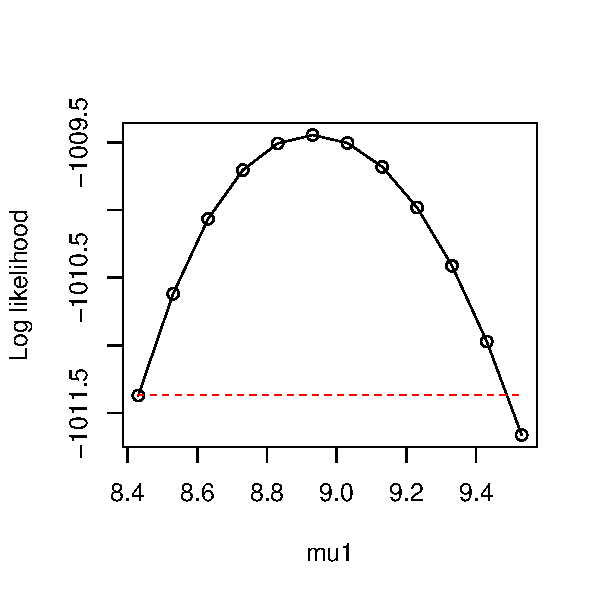
\includegraphics[width=\maxwidth]{figure/plot_profile-1} 
\end{knitrout}

\noindent Note that the profiler stops its leftward (respectively, rightward) progress
when \texttt{num\_steps\_left} (resp., \texttt{num\_steps\_right}) is exceeded, or
when the threshold is crossed, whichever happens first. Profiling is often a 
trial-and-error process of selecting values for 
\texttt{increment\_left}, \texttt{increment\_right}, \texttt{num\_steps\_left},
and \texttt{num\_steps\_right} to get complete and smooth profiles within the 
limits of available computational resources. See ``Troubleshooting: Profiles" for
additional details. 

Often one wants to plot the values of the other parameters which optimized the 
likelihood for each value of the profiled parameter. This can be done using the
\texttt{parameters} output of \texttt{profile\_likelihood}:
\begin{knitrout}
\definecolor{shadecolor}{rgb}{0.969, 0.969, 0.969}\color{fgcolor}\begin{kframe}
\begin{alltt}
\hlkwd{head}\hldef{(}\hlkwd{round}\hldef{(prof1}\hlopt{$}\hldef{parameters,} \hlnum{3}\hldef{))}
\end{alltt}
\begin{verbatim}
##    mu1  mu2 sigltil1 sigltil2 sigrtil1 sigrtil2  ctil   pd o_par1
## 1 8.43 2.38    -1.67    -1.76   -0.508   -0.236 -9.62 2.03  -6.17
## 2 8.53 2.34    -1.60    -1.80   -0.531   -0.220 -9.52 2.04  -6.15
## 3 8.63 2.30    -1.53    -1.83   -0.554   -0.202 -9.41 2.04  -6.13
## 4 8.73 2.27    -1.47    -1.85   -0.577   -0.187 -9.28 2.04  -6.11
## 5 8.83 2.24    -1.40    -1.87   -0.601   -0.171 -9.15 2.04  -6.08
## 6 8.93 2.22    -1.34    -1.90   -0.624   -0.154 -9.01 2.05  -6.06
\end{verbatim}
\begin{alltt}
\hlkwd{pairs}\hldef{(prof1}\hlopt{$}\hldef{parameters)}
\end{alltt}
\end{kframe}
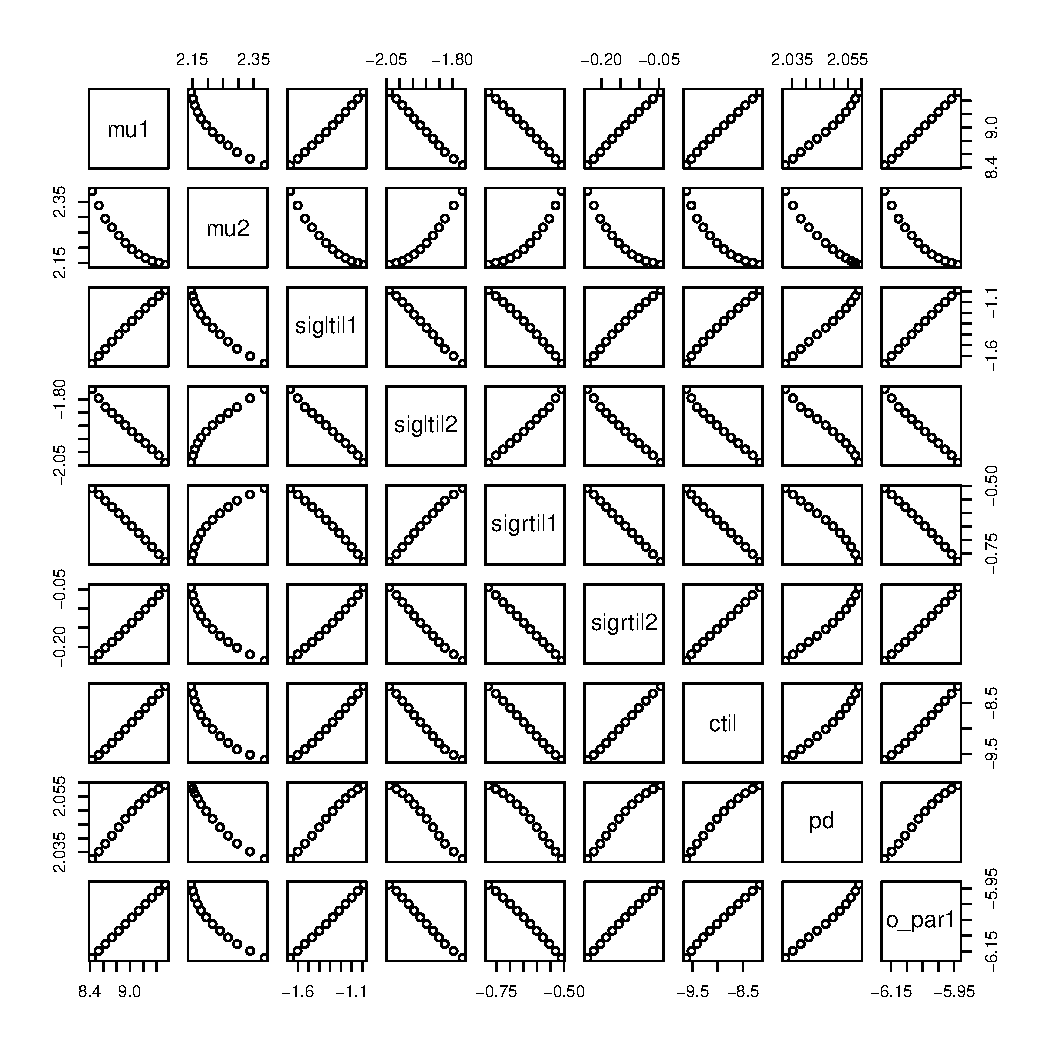
\includegraphics[width=\maxwidth]{figure/parameters_profile_output-1} 
\end{knitrout}
As a reminder, these are math-scale parameters.

Finally, the \texttt{found\_better} output of \texttt{profile\_likelihood} is
a flag which tells you whether, in the course of profiling, a higher likelihood was
found than what was previously believed to be the maximum likelihood:
\begin{knitrout}
\definecolor{shadecolor}{rgb}{0.969, 0.969, 0.969}\color{fgcolor}\begin{kframe}
\begin{alltt}
\hldef{prof1}\hlopt{$}\hldef{found_better}
\end{alltt}
\begin{verbatim}
## [1] FALSE
\end{verbatim}
\end{kframe}
\end{knitrout}
\noindent In this case, a better value was not found, which provides additional evidence that 
we had previously already succeeded in adequately maximizing the likelihood. 
If \texttt{found\_better} is \texttt{TRUE}, it means you have to go back and 
re-optimize, either with more initial conditions, or with tighter tolerances
on the optimizer used, or with a different optimizer. Although sometimes it can
be sufficient to simply re-start profiling using the parameters which were found
to yield a new highest likelihood. 

We next produce and plot all the profiles for our AIC-best model, where now the 
profiles are going to be plotted on the biological scale. Since the data are for a virtual species,
they were generated with known true parameters. We also plot the true parameter values 
together with the profiles, to verify that the fitting process has 
accurately recovered the true parameters. This exercise is complicated by the redundancy, 
discussed above, of parameters. See below for details of how to resolve that
redundancy. First make the profiles:
\begin{knitrout}
\definecolor{shadecolor}{rgb}{0.969, 0.969, 0.969}\color{fgcolor}\begin{kframe}
\begin{alltt}
\hldef{pnames} \hlkwb{<-} \hlkwd{names}\hldef{(}\hlkwd{make_mask_names}\hldef{(}\hlnum{2}\hldef{))}
\hldef{all_profiles} \hlkwb{<-} \hlkwd{list}\hldef{()}
\hlkwa{for} \hldef{(counter} \hlkwa{in} \hlnum{1}\hlopt{:}\hlkwd{length}\hldef{(pnames))}
\hldef{\{}
  \hldef{all_profiles[[counter]]} \hlkwb{<-} \hlkwd{profile_likelihood}\hldef{(}
                              \hlkwc{profile_parameter}\hldef{=pnames[counter],}
                              \hlkwc{increment_left} \hldef{=}\hlnum{0.05}\hldef{,}
                              \hlkwc{increment_right} \hldef{=} \hlnum{0.05}\hldef{,}
                              \hlkwc{num_steps_left} \hldef{=} \hlnum{50}\hldef{,}
                              \hlkwc{num_steps_right} \hldef{=} \hlnum{50}\hldef{,}
                              \hlkwc{alpha} \hldef{=} \hlnum{0.95}\hldef{,}
                              \hlkwc{optim_param_vector} \hldef{= all_optim_results[[}\hlnum{1}\hldef{]]}\hlopt{$}\hldef{par,}
                              \hlkwc{env_dat} \hldef{= env_array,}
                              \hlkwc{occ} \hldef{= occ,}
                              \hlkwc{num_threads} \hldef{=} \hlnum{7}
                            \hldef{)}
\hldef{\}}
\hlkwd{names}\hldef{(all_profiles)} \hlkwb{<-} \hldef{pnames}
\end{alltt}
\end{kframe}
\end{knitrout}

\noindent Now, to deal with the parameter redundancy, convert the 
maximum-likelihood parameters to the biological scale
and find the representation of the true parameters which is closest in parameter
space to the maximum-likelihood parameters:
\begin{knitrout}
\definecolor{shadecolor}{rgb}{0.969, 0.969, 0.969}\color{fgcolor}\begin{kframe}
\begin{alltt}
\hldef{true_parameters_bio} \hlkwb{<-} \hldef{example_1}\hlopt{$}\hldef{par_list}
\hldef{ML_parameters_bio} \hlkwb{=} \hlkwd{math_to_bio}\hldef{(all_optim_results[[}\hlnum{1}\hldef{]]}\hlopt{$}\hldef{par)}
\hldef{example_1_true_parameters_bio} \hlkwb{<-} \hlkwd{dist_between_params}\hldef{(}
  \hldef{true_parameters_bio,}
  \hldef{ML_parameters_bio,}
  \hlkwc{give_closest_rep} \hldef{=} \hlnum{TRUE}\hldef{)}\hlopt{$}\hldef{representative}
\hldef{example_1_true_parameters_bio}
\end{alltt}
\begin{verbatim}
## $mu
## [1] 9.0 2.5
## 
## $sigltil
## [1] 0.3 0.2
## 
## $sigrtil
## [1] 0.5 0.8
## 
## $ctil
## [1] -9
## 
## $pd
## [1] 0.865
## 
## $o_mat
##       [,1]   [,2]
## [1,] 0.980 -0.199
## [2,] 0.199  0.980
\end{verbatim}
\end{kframe}
\end{knitrout}

\noindent Now plot profiles. Recall we are plotting on the biological scale, so each 
parameter is transformed before the profile is plotted:
\begin{knitrout}
\definecolor{shadecolor}{rgb}{0.969, 0.969, 0.969}\color{fgcolor}\begin{kframe}
\begin{alltt}
\hlkwd{par}\hldef{(}\hlkwc{mfrow}\hldef{=}\hlkwd{c}\hldef{(}\hlnum{3}\hldef{,}\hlnum{3}\hldef{))}

\hldef{plot_tool} \hlkwb{<-} \hlkwa{function}\hldef{(}\hlkwc{x}\hldef{,} \hlkwc{y}\hldef{,} \hlkwc{thresh}\hldef{,} \hlkwc{xlab}\hldef{,} \hlkwc{true_param}\hldef{) \{}
  \hlkwd{plot}\hldef{(x, y,} \hlkwc{type}\hldef{=}\hlsng{"o"}\hldef{,} \hlkwc{xlab} \hldef{= xlab,} \hlkwc{ylab} \hldef{=} \hlsng{"Log likelihood"}\hldef{)}
  \hlkwd{lines}\hldef{(}\hlkwd{range}\hldef{(x),} \hlkwd{rep}\hldef{(thresh,} \hlnum{2}\hldef{),} \hlkwc{type} \hldef{=} \hlsng{"l"}\hldef{,} \hlkwc{lty} \hldef{=} \hlsng{"dashed"}\hldef{,} \hlkwc{col} \hldef{=} \hlsng{"red"}\hldef{)}
  \hlkwd{points}\hldef{(true_param, thresh,} \hlkwc{col} \hldef{=} \hlsng{"red"}\hldef{,} \hlkwc{pch} \hldef{=} \hlnum{20}\hldef{,} \hlkwc{cex} \hldef{=} \hlnum{2}\hldef{)}
\hldef{\}}

\hlcom{#mu1}
\hlkwd{plot_tool}\hldef{(}\hlkwc{x} \hldef{= all_profiles}\hlopt{$}\hldef{mu1}\hlopt{$}\hldef{profile}\hlopt{$}\hldef{value_math,}
  \hlkwc{y} \hldef{= all_profiles}\hlopt{$}\hldef{mu1}\hlopt{$}\hldef{profile}\hlopt{$}\hldef{loglik,}
  \hlkwc{thresh} \hldef{= all_profiles}\hlopt{$}\hldef{mu1}\hlopt{$}\hldef{threshold,}
  \hlkwc{xlab} \hldef{=} \hlsng{"mu1"}\hldef{,}
  \hlkwc{true_param} \hldef{= example_1_true_parameters_bio}\hlopt{$}\hldef{mu[}\hlnum{1}\hldef{])}

\hlcom{#mu2}
\hlkwd{plot_tool}\hldef{(}\hlkwc{x} \hldef{= all_profiles}\hlopt{$}\hldef{mu2}\hlopt{$}\hldef{profile}\hlopt{$}\hldef{value_math,}
  \hlkwc{y} \hldef{= all_profiles}\hlopt{$}\hldef{mu2}\hlopt{$}\hldef{profile}\hlopt{$}\hldef{loglik,}
  \hlkwc{thresh} \hldef{= all_profiles}\hlopt{$}\hldef{mu2}\hlopt{$}\hldef{threshold,}
  \hlkwc{xlab} \hldef{=} \hlsng{"mu2"}\hldef{,}
  \hlkwc{true_param} \hldef{= example_1_true_parameters_bio}\hlopt{$}\hldef{mu[}\hlnum{2}\hldef{])}

\hlcom{#sigltil1 - need to exp transform to get to the bio scale}
\hlkwd{plot_tool}\hldef{(}\hlkwc{x} \hldef{=} \hlkwd{exp}\hldef{(all_profiles}\hlopt{$}\hldef{sigltil1}\hlopt{$}\hldef{profile}\hlopt{$}\hldef{value_math),}
  \hlkwc{y} \hldef{= all_profiles}\hlopt{$}\hldef{sigltil1}\hlopt{$}\hldef{profile}\hlopt{$}\hldef{loglik,}
  \hlkwc{thresh} \hldef{= all_profiles}\hlopt{$}\hldef{sigltil1}\hlopt{$}\hldef{threshold,}
  \hlkwc{xlab} \hldef{=} \hlsng{"sigltil1"}\hldef{,}
  \hlkwc{true_param} \hldef{= example_1_true_parameters_bio}\hlopt{$}\hldef{sigltil[}\hlnum{1}\hldef{])}

\hlcom{#sigltil2 - need to exp transform to get to the bio scale}
\hlkwd{plot_tool}\hldef{(}\hlkwc{x} \hldef{=} \hlkwd{exp}\hldef{(all_profiles}\hlopt{$}\hldef{sigltil2}\hlopt{$}\hldef{profile}\hlopt{$}\hldef{value_math),}
  \hlkwc{y} \hldef{= all_profiles}\hlopt{$}\hldef{sigltil2}\hlopt{$}\hldef{profile}\hlopt{$}\hldef{loglik,}
  \hlkwc{thresh} \hldef{= all_profiles}\hlopt{$}\hldef{sigltil2}\hlopt{$}\hldef{threshold,}
  \hlkwc{xlab} \hldef{=} \hlsng{"sigltil2"}\hldef{,}
  \hlkwc{true_param} \hldef{= example_1_true_parameters_bio}\hlopt{$}\hldef{sigltil[}\hlnum{2}\hldef{])}

\hlcom{#sigrtil1 - need to exp transform to get to the bio scale}
\hlkwd{plot_tool}\hldef{(}\hlkwc{x} \hldef{=} \hlkwd{exp}\hldef{(all_profiles}\hlopt{$}\hldef{sigrtil1}\hlopt{$}\hldef{profile}\hlopt{$}\hldef{value_math),}
  \hlkwc{y} \hldef{= all_profiles}\hlopt{$}\hldef{sigrtil1}\hlopt{$}\hldef{profile}\hlopt{$}\hldef{loglik,}
  \hlkwc{thresh} \hldef{= all_profiles}\hlopt{$}\hldef{sigrtil1}\hlopt{$}\hldef{threshold,}
  \hlkwc{xlab} \hldef{=} \hlsng{"sigrtil1"}\hldef{,}
  \hlkwc{true_param} \hldef{= example_1_true_parameters_bio}\hlopt{$}\hldef{sigrtil[}\hlnum{1}\hldef{])}

\hlcom{#sigrtil2 - need to exp transform to get to the bio scale}
\hlkwd{plot_tool}\hldef{(}\hlkwc{x} \hldef{=} \hlkwd{exp}\hldef{(all_profiles}\hlopt{$}\hldef{sigrtil2}\hlopt{$}\hldef{profile}\hlopt{$}\hldef{value_math),}
  \hlkwc{y} \hldef{= all_profiles}\hlopt{$}\hldef{sigrtil2}\hlopt{$}\hldef{profile}\hlopt{$}\hldef{loglik,}
  \hlkwc{thresh} \hldef{= all_profiles}\hlopt{$}\hldef{sigrtil2}\hlopt{$}\hldef{threshold,}
  \hlkwc{xlab} \hldef{=} \hlsng{"sigrtil2"}\hldef{,}
  \hlkwc{true_param} \hldef{= example_1_true_parameters_bio}\hlopt{$}\hldef{sigrtil[}\hlnum{2}\hldef{])}

\hlcom{#ctil}
\hlkwd{plot_tool}\hldef{(}\hlkwc{x} \hldef{= all_profiles}\hlopt{$}\hldef{ctil}\hlopt{$}\hldef{profile}\hlopt{$}\hldef{value_math,}
  \hlkwc{y} \hldef{= all_profiles}\hlopt{$}\hldef{ctil}\hlopt{$}\hldef{profile}\hlopt{$}\hldef{loglik,}
  \hlkwc{thresh} \hldef{= all_profiles}\hlopt{$}\hldef{ctil}\hlopt{$}\hldef{threshold,}
  \hlkwc{xlab} \hldef{=} \hlsng{"ctil"}\hldef{,}
  \hlkwc{true_param} \hldef{= example_1_true_parameters_bio}\hlopt{$}\hldef{ctil)}

\hlcom{#pd - need to expit transform to get to the bio scale}
\hlkwd{plot_tool}\hldef{(}\hlkwc{x} \hldef{=} \hlkwd{expit}\hldef{(all_profiles}\hlopt{$}\hldef{pd}\hlopt{$}\hldef{profile}\hlopt{$}\hldef{value_math),}
  \hlkwc{y} \hldef{= all_profiles}\hlopt{$}\hldef{pd}\hlopt{$}\hldef{profile}\hlopt{$}\hldef{loglik,}
  \hlkwc{thresh} \hldef{= all_profiles}\hlopt{$}\hldef{pd}\hlopt{$}\hldef{threshold,}
  \hlkwc{xlab} \hldef{=} \hlsng{"pd"}\hldef{,}
  \hlkwc{true_param} \hldef{= example_1_true_parameters_bio}\hlopt{$}\hldef{pd)}

\hlcom{#o_mat - Note that this is a single parameter on the math scale, so we only}
\hlcom{#need to profile one of the matrix entries on the biological scale}
\hldef{x} \hlkwb{=} \hlkwd{sapply}\hldef{(}\hlkwc{X}\hldef{=all_profiles}\hlopt{$}\hldef{o_par1}\hlopt{$}\hldef{profile}\hlopt{$}\hldef{value_math,}
           \hlkwc{FUN}\hldef{=}\hlkwa{function}\hldef{(}\hlkwc{x}\hldef{)\{}\hlkwd{build_orthogonal_matrix}\hldef{(x)[}\hlnum{1}\hldef{,}\hlnum{1}\hldef{]\})}
\hlkwd{plot_tool}\hldef{(}\hlkwc{x} \hldef{= x,}
  \hlkwc{y} \hldef{= all_profiles}\hlopt{$}\hldef{o_par1}\hlopt{$}\hldef{profile}\hlopt{$}\hldef{loglik,}
  \hlkwc{thresh} \hldef{= all_profiles}\hlopt{$}\hldef{o_par1}\hlopt{$}\hldef{threshold,}
  \hlkwc{xlab} \hldef{=} \hlsng{"o_par1"}\hldef{,}
  \hlkwc{true_param} \hldef{= example_1_true_parameters_bio}\hlopt{$}\hldef{o_mat[}\hlnum{1}\hldef{,}\hlnum{1}\hldef{])}
\end{alltt}
\end{kframe}
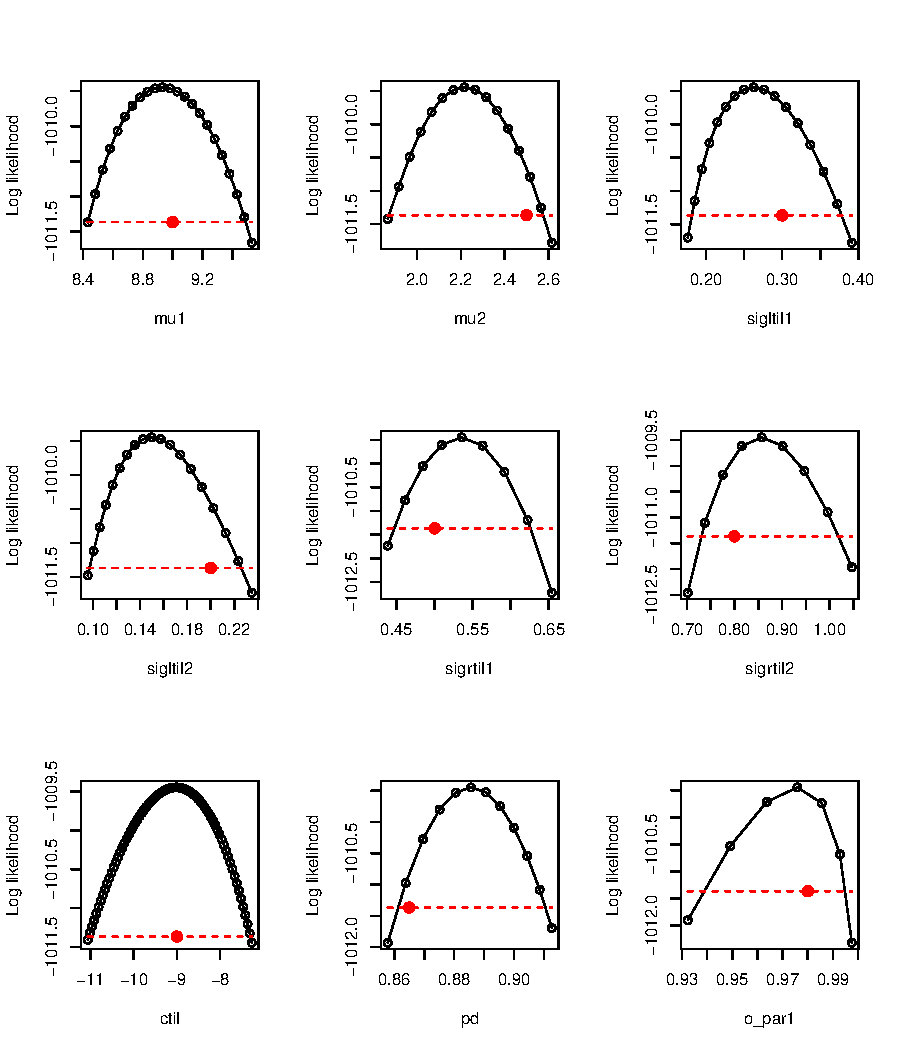
\includegraphics[width=\maxwidth]{figure/plot_all_profiles-1} 
\end{knitrout}

\noindent Note that transforming \texttt{o\_par} profiles to the biological scale
will not work the same way for more than two environmental variables because, 
in that case, there are multiple \texttt{o\_par} parameters, and they interact 
with each other in the transformation to the biological scale. In that case,
a Bayesian approach may have advantages. 

\section{Habitat suitability maps}

We have now fitted several models, selected a best one, verified that the profiles 
look good, and shown that fitting captures the true model parameters. 
Habitat suitability maps are done with 
the \texttt{vsp} function. The \texttt{vsp} function has the dual purposes of 
allowing the user to experiment with creating virtual species, and producing 
habitat suitability maps. We here use it for the latter.

\begin{knitrout}
\definecolor{shadecolor}{rgb}{0.969, 0.969, 0.969}\color{fgcolor}\begin{kframe}
\begin{alltt}
\hlcom{#plot the habitat suitability map}
\hlkwd{par}\hldef{(}\hlkwc{mfrow} \hldef{=} \hlkwd{c}\hldef{(}\hlnum{2}\hldef{,}\hlnum{3}\hldef{))}
\hldef{hab_suit} \hlkwb{=} \hlkwd{habitat_suitability}\hldef{(ML_parameters_bio, env_data)}
\hldef{terra}\hlopt{::}\hlkwd{plot}\hldef{(hab_suit,}\hlkwc{main}\hldef{=}\hlsng{"Habitat suitability"}\hldef{,}\hlkwc{xlab}\hldef{=}\hlsng{"x"}\hldef{,}\hlkwc{ylab}\hldef{=}\hlsng{"y"}\hldef{,}\hlkwc{legend}\hldef{=}\hlnum{TRUE}\hldef{)}

\hlcom{#plot the true habitat suitability map}
\hldef{hab_suit_true} \hlkwb{=} \hlkwd{habitat_suitability}\hldef{(example_1_true_parameters_bio,env_data)}
\hldef{terra}\hlopt{::}\hlkwd{plot}\hldef{(hab_suit,}\hlkwc{main}\hldef{=}\hlsng{"Habitat suitability, true"}\hldef{,}
            \hlkwc{xlab}\hldef{=}\hlsng{"x"}\hldef{,}\hlkwc{ylab}\hldef{=}\hlsng{"y"}\hldef{,}\hlkwc{legend}\hldef{=}\hlnum{TRUE}\hldef{)}

\hlcom{#plot the difference}
\hldef{terra}\hlopt{::}\hlkwd{plot}\hldef{(hab_suit}\hlopt{-}\hldef{hab_suit_true,}\hlkwc{main}\hldef{=}\hlsng{"Difference"}\hldef{,}
            \hlkwc{xlab}\hldef{=}\hlsng{"x"}\hldef{,}\hlkwc{ylab}\hldef{=}\hlsng{"y"}\hldef{,}\hlkwc{legend}\hldef{=}\hlnum{TRUE}\hldef{)}

\hlcom{#plot the species ranges assuming a threshold of 0.5}
\hldef{terra}\hlopt{::}\hlkwd{plot}\hldef{((hab_suit}\hlopt{>}\hlnum{.5}\hldef{),}\hlkwc{main}\hldef{=}\hlsng{"Species range"}\hldef{,}
            \hlkwc{xlab}\hldef{=}\hlsng{"x"}\hldef{,}\hlkwc{ylab}\hldef{=}\hlsng{"y"}\hldef{,}\hlkwc{legend}\hldef{=}\hlnum{TRUE}\hldef{)}
\hldef{terra}\hlopt{::}\hlkwd{plot}\hldef{((hab_suit_true}\hlopt{>}\hlnum{.5}\hldef{),}\hlkwc{main}\hldef{=}\hlsng{"Species range, true"}\hldef{,}
            \hlkwc{xlab}\hldef{=}\hlsng{"x"}\hldef{,}\hlkwc{ylab}\hldef{=}\hlsng{"y"}\hldef{,}\hlkwc{legend}\hldef{=}\hlnum{TRUE}\hldef{)}

\hlcom{#plot the difference}
\hldef{terra}\hlopt{::}\hlkwd{plot}\hldef{((hab_suit}\hlopt{>}\hlnum{.5}\hldef{)}\hlopt{-}\hldef{(hab_suit_true}\hlopt{>}\hlnum{.5}\hldef{),}
            \hlkwc{main}\hldef{=}\hlsng{"Difference"}\hldef{,}
            \hlkwc{xlab}\hldef{=}\hlsng{"x"}\hldef{,}\hlkwc{ylab}\hldef{=}\hlsng{"y"}\hldef{,}\hlkwc{legend}\hldef{=}\hlnum{TRUE}\hldef{)}
\end{alltt}
\end{kframe}
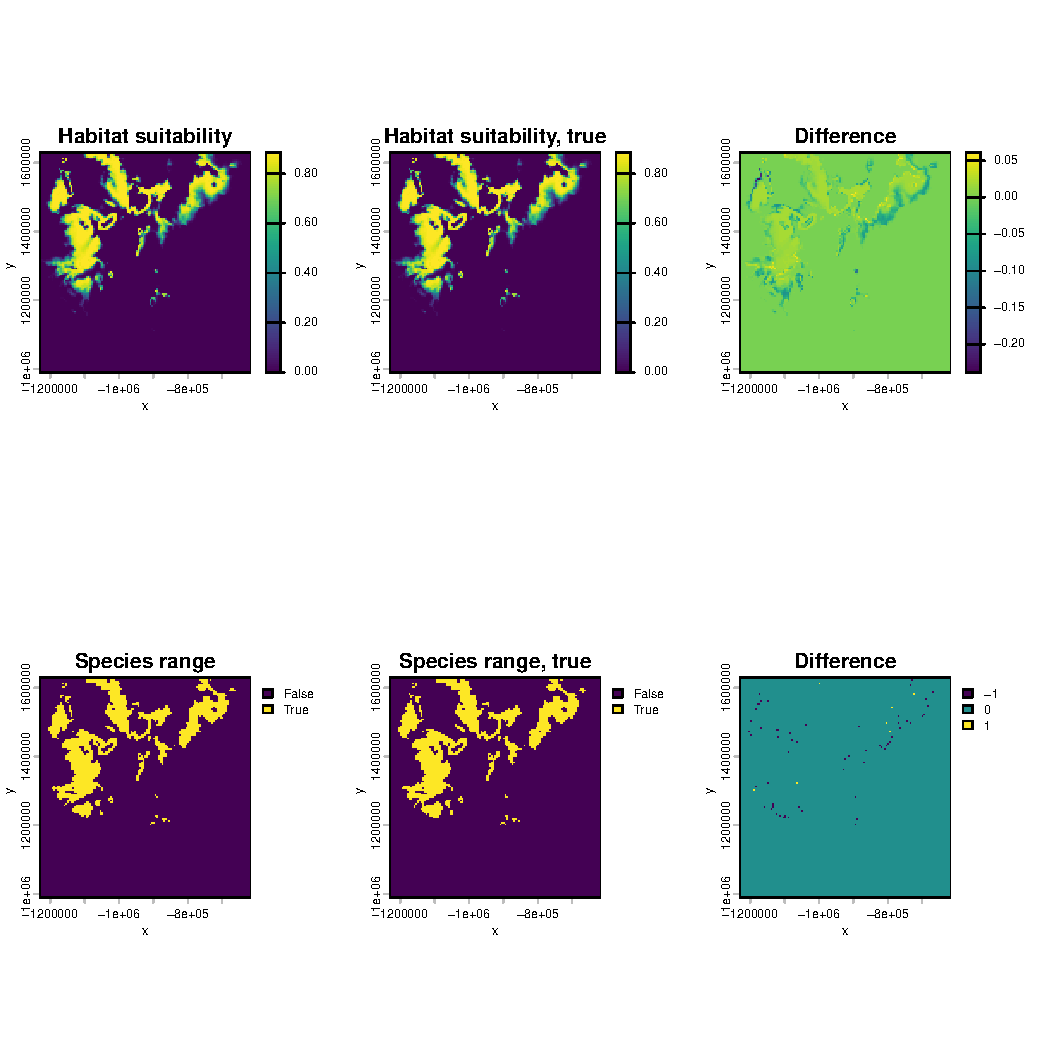
\includegraphics[width=\maxwidth]{figure/habitat_suitability-1} 
\begin{kframe}\begin{alltt}
\hlcom{#compute percent error in range}
\hldef{area} \hlkwb{=} \hlkwd{sum}\hldef{(}\hlkwd{as.data.frame}\hldef{((hab_suit_true}\hlopt{>}\hlnum{.5}\hldef{)))}
\hldef{area_setdiff} \hlkwb{=} \hlkwd{sum}\hldef{(}\hlkwd{abs}\hldef{(}\hlkwd{as.data.frame}\hldef{((hab_suit}\hlopt{>}\hlnum{.5}\hldef{)}\hlopt{-}\hldef{(hab_suit_true}\hlopt{>}\hlnum{.5}\hldef{))}\hlopt{-}\hlnum{0}\hldef{)}\hlopt{>}\hlnum{1e-1}\hldef{)}
\hldef{delta} \hlkwb{=} \hldef{(area_setdiff)}\hlopt{/}\hldef{area}
\hldef{area}
\end{alltt}
\begin{verbatim}
## [1] 2058
\end{verbatim}
\begin{alltt}
\hldef{area_setdiff}
\end{alltt}
\begin{verbatim}
## [1] 69
\end{verbatim}
\begin{alltt}
\hldef{delta}
\end{alltt}
\begin{verbatim}
## [1] 0.0335
\end{verbatim}
\end{kframe}
\end{knitrout}
 
\noindent As you can see, both the inferred habitat suitability map and the 
associated species range are similar to the true versions.

One of the main things \texttt{xsdm} is good for is assessing 
the influence of inter-annual climatic variability on species distributions,
so we also display what the habitat suitability map would look like if the value of 
each environmental variable in each location were always equal to the temporal
mean for that variable and location. We use inferred parameters.
\begin{knitrout}
\definecolor{shadecolor}{rgb}{0.969, 0.969, 0.969}\color{fgcolor}\begin{kframe}
\begin{alltt}
\hlcom{#plot the habitat suitability map again, to ease comparisons}
\hlkwd{par}\hldef{(}\hlkwc{mfrow}\hldef{=}\hlkwd{c}\hldef{(}\hlnum{2}\hldef{,}\hlnum{3}\hldef{))}
\hldef{hab_suit} \hlkwb{=} \hlkwd{habitat_suitability}\hldef{(ML_parameters_bio, env_data)}
\hldef{terra}\hlopt{::}\hlkwd{plot}\hldef{(hab_suit,}\hlkwc{main}\hldef{=}\hlsng{"Habitat suitability"}\hldef{,}\hlkwc{xlab}\hldef{=}\hlsng{"x"}\hldef{,}\hlkwc{ylab}\hldef{=}\hlsng{"y"}\hldef{,}\hlkwc{legend}\hldef{=}\hlnum{TRUE}\hldef{)}

\hlcom{#plot the habitat suitability map without variability}
\hldef{m_bio_1_ts} \hlkwb{=} \hlkwd{rep}\hldef{(m_bio_1,terra}\hlopt{::}\hlkwd{nlyr}\hldef{(bio_1))}
\hldef{m_bio_12_ts} \hlkwb{=} \hlkwd{rep}\hldef{(m_bio_12,terra}\hlopt{::}\hlkwd{nlyr}\hldef{(bio_12))}
\hldef{m_env_data}\hlkwb{=}\hlkwd{list}\hldef{(}\hlkwc{m_bio_1}\hldef{=m_bio_1_ts,}\hlkwc{m_bio_12}\hldef{=m_bio_12_ts)}
\hldef{m_hab_suit} \hlkwb{=} \hlkwd{habitat_suitability}\hldef{(ML_parameters_bio, m_env_data)}
\hldef{terra}\hlopt{::}\hlkwd{plot}\hldef{(m_hab_suit,}\hlkwc{main}\hldef{=}\hlsng{"Habitat suitability, no var"}\hldef{,}
            \hlkwc{xlab}\hldef{=}\hlsng{"x"}\hldef{,}\hlkwc{ylab}\hldef{=}\hlsng{"y"}\hldef{,}\hlkwc{legend}\hldef{=}\hlnum{TRUE}\hldef{)}

\hlcom{#plot the difference}
\hldef{terra}\hlopt{::}\hlkwd{plot}\hldef{(m_hab_suit}\hlopt{-}\hldef{hab_suit,}\hlkwc{main}\hldef{=}\hlsng{"Difference"}\hldef{,}
            \hlkwc{xlab}\hldef{=}\hlsng{"x"}\hldef{,}\hlkwc{ylab}\hldef{=}\hlsng{"y"}\hldef{,}\hlkwc{legend}\hldef{=}\hlnum{TRUE}\hldef{)}

\hlcom{#plot the species ranges assuming a threshold of 0.5}
\hldef{terra}\hlopt{::}\hlkwd{plot}\hldef{((hab_suit}\hlopt{>}\hlnum{.5}\hldef{),}\hlkwc{main}\hldef{=}\hlsng{"Species range"}\hldef{,}
            \hlkwc{xlab}\hldef{=}\hlsng{"x"}\hldef{,}\hlkwc{ylab}\hldef{=}\hlsng{"y"}\hldef{,}\hlkwc{legend}\hldef{=}\hlnum{TRUE}\hldef{)}
\hldef{terra}\hlopt{::}\hlkwd{plot}\hldef{((m_hab_suit}\hlopt{>}\hlnum{.5}\hldef{),}\hlkwc{main}\hldef{=}\hlsng{"Species range, no var"}\hldef{,}
            \hlkwc{xlab}\hldef{=}\hlsng{"x"}\hldef{,}\hlkwc{ylab}\hldef{=}\hlsng{"y"}\hldef{,}\hlkwc{legend}\hldef{=}\hlnum{TRUE}\hldef{)}

\hlcom{#plot the difference}
\hldef{terra}\hlopt{::}\hlkwd{plot}\hldef{((m_hab_suit}\hlopt{>}\hlnum{.5}\hldef{)}\hlopt{-}\hldef{(hab_suit}\hlopt{>}\hlnum{.5}\hldef{),}
            \hlkwc{main}\hldef{=}\hlsng{"Difference"}\hldef{,}
            \hlkwc{xlab}\hldef{=}\hlsng{"x"}\hldef{,}\hlkwc{ylab}\hldef{=}\hlsng{"y"}\hldef{,}\hlkwc{legend}\hldef{=}\hlnum{TRUE}\hldef{)}
\end{alltt}
\end{kframe}
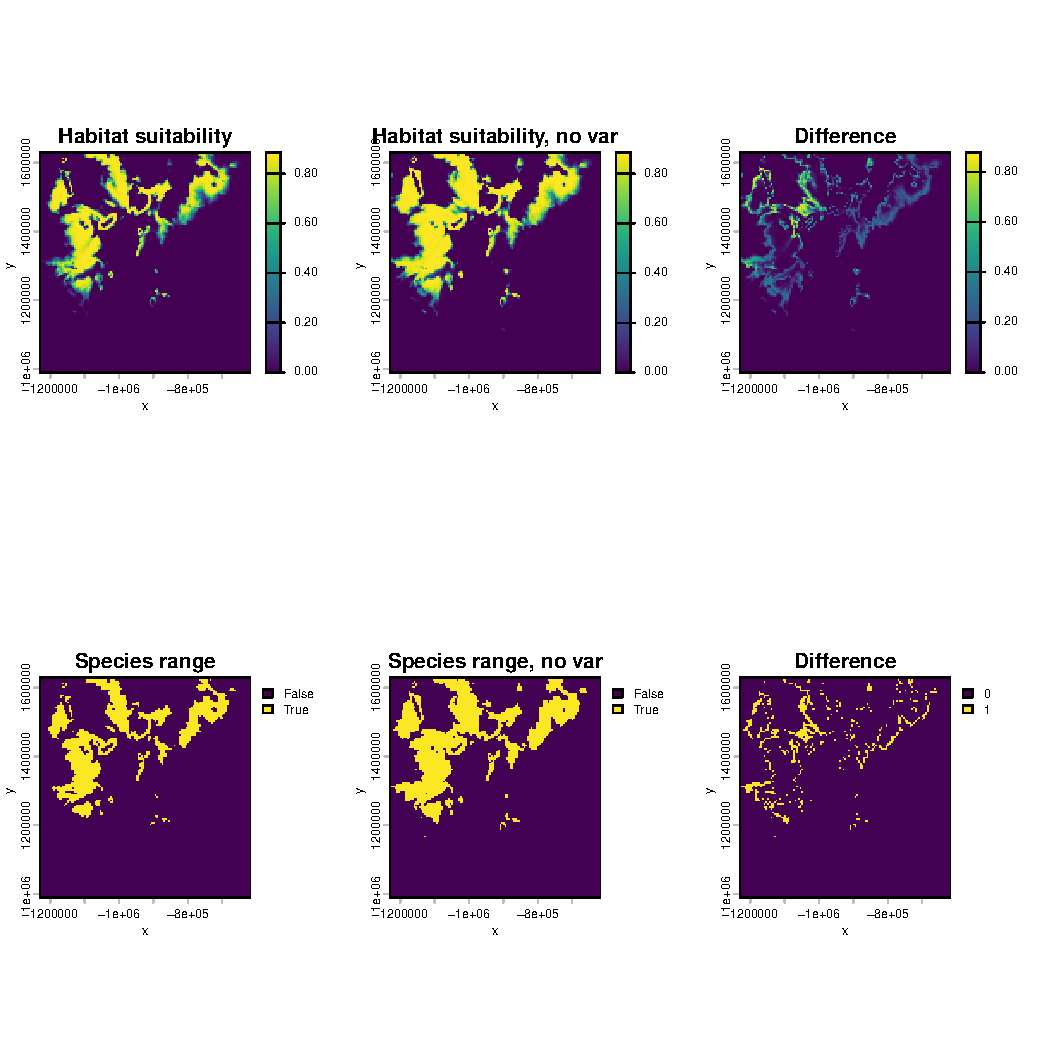
\includegraphics[width=\maxwidth]{figure/habitat_suitability_novar-1} 
\begin{kframe}\begin{alltt}
\hlcom{#compute change in area due to variability}
\hldef{area} \hlkwb{<-} \hlkwd{sum}\hldef{(}\hlkwd{as.data.frame}\hldef{((hab_suit}\hlopt{>}\hlnum{.5}\hldef{)))}
\hldef{area_novar} \hlkwb{<-} \hlkwd{sum}\hldef{(}\hlkwd{as.data.frame}\hldef{((m_hab_suit}\hlopt{>}\hlnum{.5}\hldef{)))}
\hldef{delta_area} \hlkwb{<-} \hldef{(area_novar}\hlopt{-}\hldef{area)}\hlopt{/}\hldef{area_novar}
\hldef{area}
\end{alltt}
\begin{verbatim}
## [1] 2003
\end{verbatim}
\begin{alltt}
\hldef{area_novar}
\end{alltt}
\begin{verbatim}
## [1] 2716
\end{verbatim}
\begin{alltt}
\hldef{delta_area}
\end{alltt}
\begin{verbatim}
## [1] 0.263
\end{verbatim}
\end{kframe}
\end{knitrout}

\noindent So we see variability reduces area by 26.25\%
for this virtual species.

\section{Interpreting model parameters}

We would like to interpret the the parameters of the fitted model to say 
what we can about how the species responds to the environment. This is rendered a bit 
more challenging due to the parameter reduction step which was carried 
out for the model to eliminate structural non-identifiability (see ``The xsdm model'' 
for details). The function \texttt{interpret\_parameters} helps with this, displaying
plots which describe the inferred growth-environment function (the relationship
between the environment, $\vec{e}_t$, in a given year in a location and the 
annual net growth rate, $\lambda_t$). For instance, for our example,
the contours of that function are determined, though their heights are not determined.
The contours are enough to tell the user what the optimal environment is for the
species, and how sensitive annual net growth is to departures from this optimum
for each environmental variable, relative to the other environmental variables:
\begin{knitrout}
\definecolor{shadecolor}{rgb}{0.969, 0.969, 0.969}\color{fgcolor}\begin{kframe}
\begin{alltt}
\hlkwd{interpret_parameters}\hldef{(}\hlkwc{param_list} \hldef{= ML_parameters_bio,}
                     \hlkwc{plot_indices} \hldef{=} \hlkwd{c}\hldef{(}\hlnum{1}\hldef{,}\hlnum{2}\hldef{),}
                     \hlkwc{env_dat} \hldef{= env_array,}
                     \hlkwc{occ} \hldef{= example_1}\hlopt{$}\hldef{occ_df}\hlopt{$}\hldef{presence)}
\end{alltt}
\end{kframe}

\includegraphics[width=\maxwidth]{figure/interpret_parameters-1} 
\end{knitrout}

\noindent The points displayed here are all values of the environmental variables, 
in any year, in locations for which the species was detected (left) or assumed
absent (right). One can see that growth is inferred to be more sensitive to low temperatures
(leftward departures of environmental variable 1 from the optimum) than it is
to high temperatures (rightward departures); and growth is more sensitive to drought
(downward departures of environmental variable 2 from the optimum) than it is to
abundant rainfall (upward departures). One can see that, as expected, the environment
is more suitable for population growth, according to the inferred growth-environment
function, in locations for where the species was observed. One can see that, 
even in locations found to be unsuitable for the species (right panel),
there were plenty of individual years for which environmental conditions promoted
growth in that year, demonstrating the importance of interannual variability.

Now we plot the same thing for the true parameters:
\begin{knitrout}
\definecolor{shadecolor}{rgb}{0.969, 0.969, 0.969}\color{fgcolor}\begin{kframe}
\begin{alltt}
\hlkwd{interpret_parameters}\hldef{(}\hlkwc{param_list} \hldef{= example_1}\hlopt{$}\hldef{par_list,}
                     \hlkwc{plot_indices}\hldef{=}\hlkwd{c}\hldef{(}\hlnum{1}\hldef{,}\hlnum{2}\hldef{),}
                     \hlkwc{env_dat} \hldef{= env_array,}
                     \hlkwc{occ} \hldef{=  example_1}\hlopt{$}\hldef{occ_df}\hlopt{$}\hldef{presence}
                     \hldef{)}
\end{alltt}
\end{kframe}

\includegraphics[width=\maxwidth]{figure/interpret_parameters_true-1} 
\end{knitrout}

\noindent Results were quite similar. Plots against one environmental variable
are also possible, holding the other one at optimal values. See the documentation
of \texttt{interpret\_parameters} for details.

\end{document}
